%\documentclass[a4paper,12pt,twoside]{report}
\documentclass[11pt,a4paper,UKenglish,twoside]{book} % openanyopenright
% macros.sty  Macros for mathematics, Dag Fritzson 92-07-29
\typeout{Document style `macros':  Macros for mathematics, version 92-07-29}
%
% Fourth order tensor, second order tensor (matrix), and first order tensor (vector)
\newcommand{\T}[1]{\mbox{\boldmath $\underline{#1}$}} % Forth order tensor
\newcommand{\M}[1]{\mbox{\boldmath ${#1}$}}           % Second order tensor
\newcommand{\V}[1]{\mbox{\boldmath $\vec{#1}$}}       % First order tensor
%
% Unit vectors, and zero vector
\newcommand{\eHAT}{\mbox{$\bf\hat{e}$}}
\newcommand{\aHAT}{\mbox{$\bf\hat{a}$}}
\newcommand{\IHAT}{\mbox{$\bf\hat{I}$}}
\newcommand{\vzero}{\mbox{\bf 0}}
%
% Versions of the \frac command with different font sizes
\newcommand{\mbfrac}[2]{\mbox{$\frac{#1}{#2}$}}
\newcommand{\nofrac}[2]{\frac{\mbox{\normalsize${#1}$}}
                             {\mbox{\normalsize${#2}$}}}
\newcommand{\smfrac}[2]{\mbox{\small$\frac{#1}{#2}$}}
\newcommand{\fofrac}[2]{\frac{\mbox{\footnotesize${#1}$}}
                             {\mbox{\footnotesize${#2}$}}}
\newcommand{\scfrac}[2]{\frac{\mbox{\scriptsize${#1}$}}
                             {\mbox{\scriptsize${#2}$}}}
%
% Superscript and subscript
\newcommand{\ri}[1]{\mbox{{\scriptsize {#1}}}} % Two functions to get correct font
\newcommand{\rii}[1]{\mbox{{\tiny {#1}}}}      % for labels in subscript
\newcommand{\regtrademark}{$^{\hspace{1pt}\mbox{\tiny{R}}\hspace{-2.5mm}{\bigcirc}}$}
\newcommand{\trademark}{$^{\hspace{1pt}\mbox{\tiny{TM}}}$}
\newcommand{\inch}{\mbox{$^{\prime\prime}$}}
\newcommand{\foot}{\mbox{$^{\prime}$}}
\newcommand{\degrees}{\mbox{$^{\circ}$}}
\newcommand{\twoprime}{\prime\prime}
\newcommand{\threeprime}{\prime\prime\prime}
%
% Matrix(3x3), vector(3), vector(2) in component form

% vector (3)
\newcommand{\vcomp}[3]{\left[\begin{array}{c}   
                       {#1} \\
                       {#2} \\
                       {#3}
                     \end{array}\right]} 

% matrix (3x3)
\newcommand{\mcomp}[9]{\left[\begin{array}{ccc} 
                       {#1} & {#2} & {#3} \\
                       {#4} & {#5} & {#6} \\
                       {#7} & {#8} & {#9} 
                     \end{array}\right]} 

\newcommand{\mcomptwo}[4]{\left[\begin{array}{cc}
                       {#1} & {#2} \\
                       {#3} & {#4}
                     \end{array}\right]}

% vector (2)
\newcommand{\vcomptwo}[2]{\left[\begin{array}{c} 
                       {#1} \\
                       {#2}
                     \end{array}\right]} 
%
% For computer variables or functions the font tt (Courier) should be used.
\newcommand{\C}[1]{\mbox{\tt #1}}           % The tt font for variable or function.
%
% The arccos function
\newcommand{\arccot}{\mbox{arccot}}
%
% Partial derivatives in rational notation

% First order derivative
\newcommand{\D}[2]{\mbox{$\nofrac{\partial {#1}}{\partial {#2}}$}}

% Second order derivative 
\newcommand{\Dii}[2]{\mbox{$\nofrac{\partial^{2} {#1}}    
                                   {\partial {#2}^{2}}$}}

% Mixed derivative
\newcommand{\Dij}[3]{\mbox{$\nofrac{\partial^{2} {#1}}         
                                   {\partial {#2}\partial{#3}}$}}

% Third order derivative 
\newcommand{\Diii}[2]{\mbox{$\nofrac{\partial^{3} {#1}}    
                                   {\partial {#2}^{3}}$}}
\newcommand{\FD}[2]{\mbox{$\nofrac{ d {#1}}{ d {#2}}$}}
\newcommand{\FSD}[2]{\mbox{$\nofrac{ d^{2} {#1}}{ d {#2}^{2}}$}}
\newcommand{\abs}[1]{\vert #1 \vert}
%
% Derivatives with respect to time (dot notation)
%\def\stackrel#1#2{\mathrel{\mathop{#2}\limits^{#1}}}   % Internal definition
\def\putunder#1#2{\mathrel{\mathop{#1}\limits_{#2}}}    % Internal definition
\def\putunderr#1#2{\mathclose{\mathop{#1}\limits_{#2}}} % Internal definition
\def\putunderl#1#2{\mathopen{\mathop{#1}\limits_{#2}}}  % Internal definition
\newcommand{\dt}[1]{\mbox{$\dot{#1}$}}   % First order derivative
\newcommand{\ddt}[1]{\mbox{$\ddot{#1}$}} % Second order derivative
%
% Total derivatives in rational notation
\newcommand{\Dt}[2]{\mbox{$\nofrac{d {#1}}{d^{\mbox{}}{#2}}$}} % First order derivative
\newcommand{\DDt}[2]{\mbox{$\nofrac{d^{2} {#1}}{d {#2}^{2}}$}} % Second order derivative
%
% Special notation to give the coordinate system in which the derivative is taken

% For dot notation
\newcommand{\reld}[1]{\mbox{$\putunderr{\left|\mbox{}\right.}{#1}$}}  

% For rational notation
\newcommand{\relD}[1]{\mbox{$\putunderr{{\left|\frac{\mbox{}}         
                                                    {\mbox{}}\right.}}{#1}$}}

%\newcommand{\dtrel}[2]{\mbox{$\dot{#1}\putunderr{\left|\mbox{}\right.}{#2}$}}
%\newcommand{\ddtrel}[2]{\mbox{$\ddot{#1}\putunderr{\left|\mbox{}\right.}{#2}$}}
%
%%
% A certain type of Postscript and special command. Kept for backward
% compability. Use epsf.sty now.
\newcounter{skallpostscriptritas}
\setcounter{skallpostscriptritas}{1}
\newcounter{skallcgipostritas}
\setcounter{skallcgipostritas}{1}
\newcommand{\mypath}{}
\newcommand{\post}[5]{{
% arg1 filename of postscript file
% arg2 vsize in mm
% arg3 hoffset in mm
% arg4 voffset in mm
% arg5 scale
 \vspace*{#2 mm}
 \ifnum\value{skallpostscriptritas}=1
 \special{psfile=\mypath#1  hoffset=#3  voffset=#4  hscale=#5  vscale=#5 }
 \fi
}}
\newcommand{\cgipost}[6]{{
% arg1 filename of postscript file
% arg2 hsize   in mm
% arg3 vsize   in mm
% arg4 hoffset in mm
% arg5 voffset in mm
% arg6 scale
\begin{center}
\begin{minipage}{#2mm}
\vspace*{#3mm}
\ifnum\value{skallcgipostritas}=1
 \special{psfile=\mypath#1 hoffset=#4 voffset=#5 hscale=#6 vscale=#6}
\fi
\hspace*{#2mm}
\end{minipage}
\end{center}
}}
%
% Default page settings
\setlength{\textwidth}{142mm}
\setlength{\oddsidemargin}{2.6mm}
\setlength{\evensidemargin}{14.6mm}
\setlength{\topmargin}{-13.4mm}
\setlength{\textheight}{220mm}
\setlength{\headheight}{19mm}
\setlength{\headsep}{9mm}
%\setlength{\footskip}{7mm}
%\setlength{\footheight}{7mm}
%

\usepackage[ansinew]{inputenc} %signs
\usepackage[english]{babel} 
%\usepackage[T1]{fontenc} %  fonte (output) enable when printing the report
\usepackage{graphicx} % insert image
\usepackage{subfigure}
\usepackage[numbers]{natbib}
%\usepackage{verbatim} %
\usepackage{shortvrb} % use to create a easy |
\usepackage{amsmath,amssymb,amstext,latexsym} % math symbols
\usepackage{textcomp,calc}
\usepackage{mathtools} % mathmatics
\usepackage{marvosym}
\usepackage{lipsum}
\usepackage{pdfpages}
\usepackage[font=small,labelfont=bf]{caption}
\usepackage{titlesec}
\usepackage{afterpage} % Clear floats after each page
\usepackage{datetime}
\usepackage{tikz}

\usepackage{eepic}
\usepackage{epic}
\usepackage{rotating}


\titleformat{\chapter}[display]{\normalfont\Large\bfseries\color[rgb]{0,0.4,0.796078431372549}}{\normalfont\huge\bfseries\chaptername \space \thechapter}{16pt}{\Huge}
\titleformat{\part}[display]{\centering\normalfont\Large\bfseries\color[rgb]{0,0.4,0.796078431372549}}{\centering\normalfont\huge\bfseries\partname~\thepart}{16pt}{\Huge}
\titleformat{\section}{\normalfont\Large\bfseries\color[rgb]{0,0.4,0.796078431372549}}{\thesection}{1em}{}
\titleformat{\subsection}{\normalfont\large\bfseries\color[rgb]{0,0.4,0.796078431372549}}{\thesubsection}{1em}{}
\titleformat{\subsubsection}{\normalfont\normalsize\bfseries\color[rgb]{0,0.4,0.796078431372549}}{\thesubsubsection}{1em}{}
\titleformat{\paragraph}{\normalfont\normalsize\bfseries\color[rgb]{0,0.4,0.796078431372549}}{\theparagraph}{1em}{}
\titleformat{\subparagraph}{\normalfont\normalsize\bfseries\color[rgb]{0,0.4,0.796078431372549}}{\thesubparagraph}{1em}{}


\usepackage{longtable}
\usepackage{multirow}
\usepackage{thesislayout}

%_______________________________________________________________________________________
\makeatletter
\renewcommand\fps@figure{htbp}
\renewcommand\fps@table{htbp}
\makeatother
%_______________________________________________________________________________________


%__________________________________________________________________

%NOTE algorithm MUST be loaded after hyperref or things DO break!!
%The counter for algorithms is not recognized by hyperref.
\usepackage{algorithm,algorithmic}
\usepackage{pstricks} %basic pstricks support
\usepackage{multirow}

%_______________________________________________________________________________________


%table colors
\usepackage{colortbl} %til farver i tabeller
\usepackage{array,booktabs,color}

% link colors
\usepackage{url} 
%\usepackage[colorlinks,linkcolor={black},citecolor={black},urlcolor={black},linktocpage]{hyperref}

\newcommand*{\rc}{
  \textcolor[rgb]{0,0.4,0.796078431372549}}

%_______________________________________________________________________________________


%Margin

\usepackage[innermargin=3.7cm,outermargin=3.7 cm,top=3.5cm,bottom=3.5cm]{geometry}

%_______________________________________________________________________________________

%NEW COMMANDOS
%\image{!hbtp}{0.9}{quadruple-tank.png}{figuretext}{tableofcontentstext}

\newcommand*{\image}[5]{%image{htb}{0.9}{filnavn}{caption}
\begin{figure}[#1]
    \centering
    \includegraphics[width=#2\textwidth]{./figs/#3}
    \caption[#5]{#4}\label{fig:#3}
\end{figure}
}


%\eq{equation}{label}
\newcommand*{\eq}[2]{
\begin{equation}
    #1
   \label{eq:#2}
\end{equation}
}

%_______________________________________________________________________________________
%COMMANDOS
\addto\captionsenglish{\renewcommand*\bibname{\rc{Bibliography}}}
\addto\captionsenglish{\renewcommand*\contentsname{\rc{List of Contents}}}
\addto\captionsenglish{\renewcommand*\listfigurename{\rc{List of Figures}}}
\addto\captionsenglish{\renewcommand*\listtablename{\rc{List of Tables}}}

%_______________________________________________________________________________________
%PDF Property

\usepackage{hyperref}
\hypersetup{pdftitle={Transmission Line Modeling},
                pdfauthor={SKF},
                pdfsubject={TLM},
                colorlinks,
                }


%_______________________________________________________________________________________
\parindent=14pt

\begin{document}

\frontmatter

\makefrontpage
\thispagestyle{empty}

%\tableofcontents
%\listoffigures
%\listoftables
\mainmatter
\tableofcontents

%\chapter{Background%}
\chapter{Co-Simulation Framework}
A general framework for meta-model based co-simulations has previously
been designed~\cite{Siemers+Nakhimovski+Fritzson-05}. The design goals
for the simulation part of the framework were portability, simplicity
to incorporate new simulation tools, and computational efficiency.
These goals were realized by defining the following concepts and
interfaces:

\textbf{External interface.} A named point on a mechanical object
where position and velocity can be evaluated and reaction load (force
and moment) applied. To guarantee numerical stability when utilising
different numerical solvers in the co-simulation, only interfaces based
on the {\em transmission line modelling} method, see Section~\ref{secTLMtheory}, are
currently supported.

%\item
\textbf{Simulation manager.} The central simulation engine. It is a stand alone
program that reads an XML definition of the coupled simulation.  It
then starts \emph{external model simulations} and provides the
communication bridge between the running simulations. The external
models only communicate with the simulation manager which acts as a
broker marshalling information between the external models. Simulation
manager sees every external model as a black box having one or several
external interfaces. The information is then forwarded between
external interfaces belonging to different external
models. Additionally the simulation manager opens a network port for
monitoring all communicated data.

%\item
\textbf{Interface plug-in.} A small C++ library having a single
abstract class representing external interface for a specific
simulation tool. The interface plug-in can be seen by an external
model simulator as an external load that depends on position, velocity
and time. The implementation of the plug-in handles the necessary
communications with the simulation manager. It also handles necessary
coordinate system transformations into the global meta-model inertial
system. All positions and velocities are transformed from the
external-model (simulation-tool specific) inertial system to the
global meta-model inertial system. All reaction loads are translated
back into the local inertial system. This constant transformation is
stored in the meta-model and sent to the corresponding interface
plug-in on simulation start up.
%\item

\textbf{External model simulator.} Any simulation program that has incorporated
the interface plug-in as a part of its model. A small script that
takes the general parameters as input and starts the specific
simulation tool is an additional requirement. This intermediate step
is necessary since the simulation manager needs a common way
to start all the components and each tool might have some specific
start procedures.
%\end{itemize}

\section{Requirements on External Model Simulators}
\label{sec:requirements}
External models are associated with specialised simulation tools. Even
though many simulation tools have interfaces to external functions, the
interfaces differ between tools. Therefore it is first necessary that
a software developer who is familiar with the particular tool
architecture, designs and implements the {\em external interface} for
each tool. That is, to create a tool specific wrapper for the {\em
interface plug-in} of the simulation framework.

The following functionality is required from all simulation
tools that implement the interface plug-in and want to participate in
co-simulation:
\begin{itemize}
\item Possibility to start simulation externally or in batch mode.
  The developer of the tool specific interface must provide a start up
  program. This is used by the simulation manager to set-up global
  simulation parameters, that is, start time, end time, and max time
  step for each co-simulation participant. Regarding the maximum time
  step length: The current co-simulation communication protocol is
  based on the {\em transmission line modelling} method, see
  Section~\ref{secTLMtheory} for details. This method requires a
  certain communication time control, i.e., time steps need to be
  within a physically motivated limit.

\item Possibility to integrate the {\em interface plug-in} into the tool specific
	adaptor. Note that the tool independent part of the plug-in is
	implemented in C++. Some tools require external functions to
	be implemented in, e.g., C or Fortran. In such cases the C++
	code can be invoked from a C or Fortran function.

\item Ability to deliver position, orientation and velocity of a
	point to the {\em interface plug-in} and receive the reaction
	load (force and moment) to be applied at this point.

\item Ability to send information about the taken solver steps to the
  interface. This is important for variable time step solvers. Data is
  send from one co-simulation party to the other when a time step is
  completed, that is, if the solver, after many iterations, decided
  what step it will take next. This information needs to be send to
  the TLMPlugin.

\item Correct handling of shutdown signals coming from the tool specific
	wrapper. In some cases the {\em simulation manager} needs to
	take down the simulation tool in a controlled way. This can be
	achieved by a tool specific API ({\em Application Programming
	Interface}) call or simply handling of exit signals.

\end{itemize}

Additionally it is desirable that the simulation tool can export
surface geometry (graphics) for visualisation in the meta-model
environment. Surface geometry is not required for correct
meta-modelling but beneficial for visual model verification.

%These requirements are met by all the simulation tools investigated in
%this work, see Table~\ref{tab:SimTools}

Most of the commonly used simulation tools offer some kind of external
connection either through inter process communication (IPC), e.g.,
network sockets or remote procedure calls, or an application
programming interface (API). Both options are acceptable for
implementation of the interface plug-in as long as they fulfil the
requirements above. The main focus of this work is on transient
simulations of mechanical systems. Simulation tools that are of
interest for this work are pure mechanical system and multi physics
tools. All of the tools that have been considered for integration into
the co-simulation framework comply with the requirements, some of the
tools are shown in Table~\ref{tab:SimTools}. Interface plug-ins for
SKF's BEAST, SKF's Orpheus, MSC.ADAMS, Matlab/Simulink, and Modelica
have successfully been implemented and tested.

\begin{table}
\begin{center}
\caption{\em List of potential simulators considered for TLM
co-simulation. Possible implementation and type of the interface
plug-in are also shown. }
\vspace*{1mm}
\begin{tabular}{||c|c|c|c||}

\hline
Simulator & Implementation  & Interface \\
\hline
\hline
BEAST   & C++     &  TLM enabled control points \\
(SKF in-house)	& implementation & (coordinate-systems)\\
\hline
%Orpheus         & C++            &   \\
%(SKF in-house)	& implementation &   \\
%\hline
MSC.ADAMS  & C wrapper DLL	    &  General force with \\
	   & (dynamic link library) &  sub-routine call  \\
\hline
Matlab/Simulink  & C wrapper & S-function interface \\
\hline
Modelica  & C or Fortran wrapper & External function interface\\
\hline
Simpack  & Fortran wrapper & SIMPACK User routine  \\
\hline
%Ansys  &  &  & No\\

\end{tabular}
\label{tab:SimTools}
\end{center}
\end{table}

\section{External Model startup}
The requirements on the external model simulators, that is, the
simulation tools that are supposed to participate in a meta-model
simulation are defined above, see Section~\ref{sec:requirements}. One
requirement specifies that the simulation tool should be executable in
batch mode, this is, the simulation manager should be able to start
the simulation tool and pass certain parameters to the program.

The developer of the simulation tool specific adapter (TLMPlugin)
should provide a start-up program/script that accepts the following
command line parameters:
\begin{itemize}
\item \emph{Model} - the name of the sub-model as presented in the
meta-model definition. This name typically corresponds to the
component specific input file name.
\item {FromTime} - start time for the simulation.
\item {ToTime} - end time for the simulation.
\item {Step} - maximum time step allowed for the simulation. This depends on
the minimum TLM delay associated with one of the TLM links connected to the sub-model.
\item {Server:port} - name of the host machine running TLM manager application and
the TCP/IP port where TLM server is listening. This information is required for
TLM-plugin initialization. It is provided by the TLM manager as the last
argument to the start script.
\end{itemize}

A sample OpenModelica Linux start-up script could look like this:
{\scriptsize
\begin{verbatim}
#!/bin/sh
# OpenModelica TLM start-up script
# Start with 6 arguments:
# 1 XModelName (XModel directory)
# 2 start-time
# 3 end-time
# 4 max-time-step
# 5 server-name:port
# 6 model-file

OpenModelicaPath=/opt/OpenModelica
TLMModelicaPath=/opt/OpenModelica/TLMPlugin/Modelica
OMC_Cmd="${OpenModelicaPath}/bin/omc"
TLMCONFIGFILE=tlm.config
LD_LIBRARY_PATH=${OpenModelicaLibPath}/lib

echo Writing caseID $1 and server name $5 to file $TLMCONFIGFILE
echo $1 > $TLMCONFIGFILE
echo $5 >> $TLMCONFIGFILE
echo $2 >> $TLMCONFIGFILE
echo $3 >> $TLMCONFIGFILE
echo $4 >> $TLMCONFIGFILE

MOSFILE=$1.mos
MODELNAME=`basename $6 .mo`
INTERVAL_STR="($3-$2)/($4)"
INTERVAL_STR="scale=8;${INTERVAL_STR/e/*10^}"
INTERVALS=`echo $INTERVAL_STR | bc`

echo Writing $MOSFILE
echo // Autogenerated modelica script for TLM cosimulation > $MOSFILE
echo "setEnvironmentVar( \"MODELICAUSERCFLAGS\", \\
                         \"-I${TLMModelicaPath} \\
                         -L${TLMModelicaPath}/${ABI}\");" >> $MOSFILE
echo "loadModel(Modelica);" >> $MOSFILE
echo "loadFile(\"${TLMModelicaPath}/TLM.mo\");" >> $MOSFILE
echo "loadFile(\"$6\");" >> $MOSFILE
echo "getErrorString();" >> $MOSFILE
echo "checkModel($MODELNAME);" >> $MOSFILE
echo "getErrorString();" >> $MOSFILE
echo "translateModel($MODELNAME);" >> $MOSFILE
echo "getErrorString();" >> $MOSFILE
echo "simulate($MODELNAME, startTime=$2, \\
                           stopTime=$3, \\
                           numberOfIntervals=$INTERVALS, \\
                           method=\"dassl\", \\
                           outputFormat=\"plt\");" >> $MOSFILE
echo "getErrorString();" >> $MOSFILE

echo Starting OpenModelica with: $OMC_Cmd $MOSFILE
$OMC_Cmd $1.mos > $1.simlog

\end{verbatim}
}

A sample OpenModelica Windows batch start-up script could look like this:
{\scriptsize
\begin{verbatim}
echo off
REM OpenModelica TLM start-up script
REM Start with 6 arguments:
REM 1 XModelName (XModel directory)
REM 2 start-time
REM 3 end-time
REM 4 max-time-step
REM 5 server-name:port
REM 6 model-file

set OpenModelicaPath=C:/OpenModelica1.8.1
set OMC_Cmd=%OpenModelicaPath%/bin/omc.exe
set TLMCONFIGFILE=tlm.config

cd %1

echo Writing caseID %1 and server name %5 to file %TLMCONFIGFILE%
echo %1 > %TLMCONFIGFILE%
echo %5 >> %TLMCONFIGFILE%
echo %2 >> %TLMCONFIGFILE%
echo %3 >> %TLMCONFIGFILE%
echo %4 >> %TLMCONFIGFILE%

set MOSFILE=%1.mos
for /F %%I in ("%6") do set MODELNAME=%%~nI
for /F %%I in ("%Mofile%") do set MODELNAME_WITH_MO=%%I
calc (%3-%2)/%4
call result.bat
set INTERVALS=%res%

echo Writing %MOSFILE%
echo // Autogenerated modelica script for TLM cosimulation > %MOSFILE%
echo setEnvironmentVar("MODELICAUSERLFLAGS", \\
                       "-L/c/OpenModelica/sources/TLMPlugin/Modelica/WINDOWS32"); >> %MOSFILE%
echo loadModel(Modelica); >> %MOSFILE%
echo loadFile("%6"); >> %MOSFILE%
echo checkModel(%MODELNAME%); >> %MOSFILE%
echo simulate(%MODELNAME%, startTime=%2, stopTime=%3, \\
              numberOfIntervals=%INTERVALS%, \\
              tolerance=0.000001, \\
              method="euler", \\
              outputFormat="plt", \\
              variableFilter="x"); >> %MOSFILE%

echo Starting OpenModelica with: %OMC_Cmd% %MOSFILE%
%OMC_Cmd% %1.mos > %1.simlog
\end{verbatim}
}

NOTE, that the above approach requires that the Modelica TLMPlugin
reads the file ``\$TLMCONFIGFILE'' in order to get the TLM parameters.

\section{Meta-Model Simulation}
A meta-model simulation environment has been created that is based on
the previously defined co-simulation framework. The system design of
the environment is shown in Figure~\ref{fig:SystemDesign}. The
environment provides:
\begin{itemize}
\item Generality, due to the general framework
	that allows for integration of many different simulation
	tools.
\item A generic method of co-simulation based on a meta-model.
\item A general method of external model execution, i.e., all
	simulation tools involved are executed. Generality is achieved
	by a platform independent start up command that takes care of
	possible actions, i.e., remote login, file transfer, or set up
	of a parallel simulation environment.
\item Communication and data transfer between the different external
	models.
\item Data monitoring for analysis and post processing.
\item Controlled simulation termination where all external models are
	taken down in a correct way. This includes error handling due
	to external model failure or network problems.
\end{itemize}

\begin{figure}[ht]\begin{center}
    %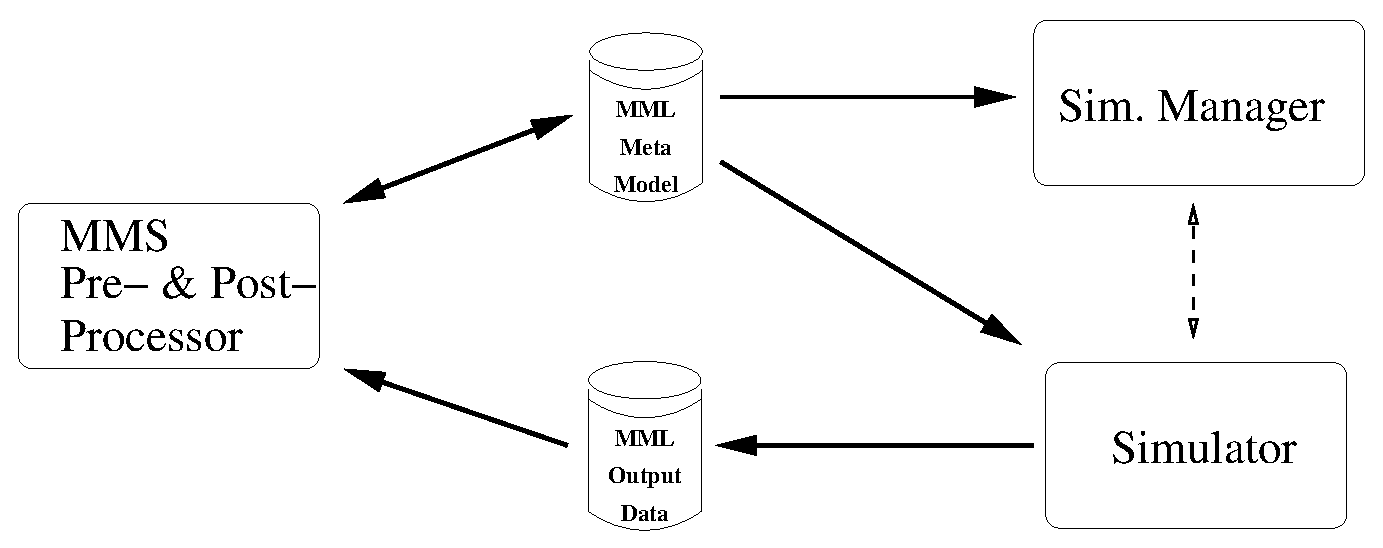
\epsfig{file=MetaModelSysDesign2.eps, width=10cm}
   {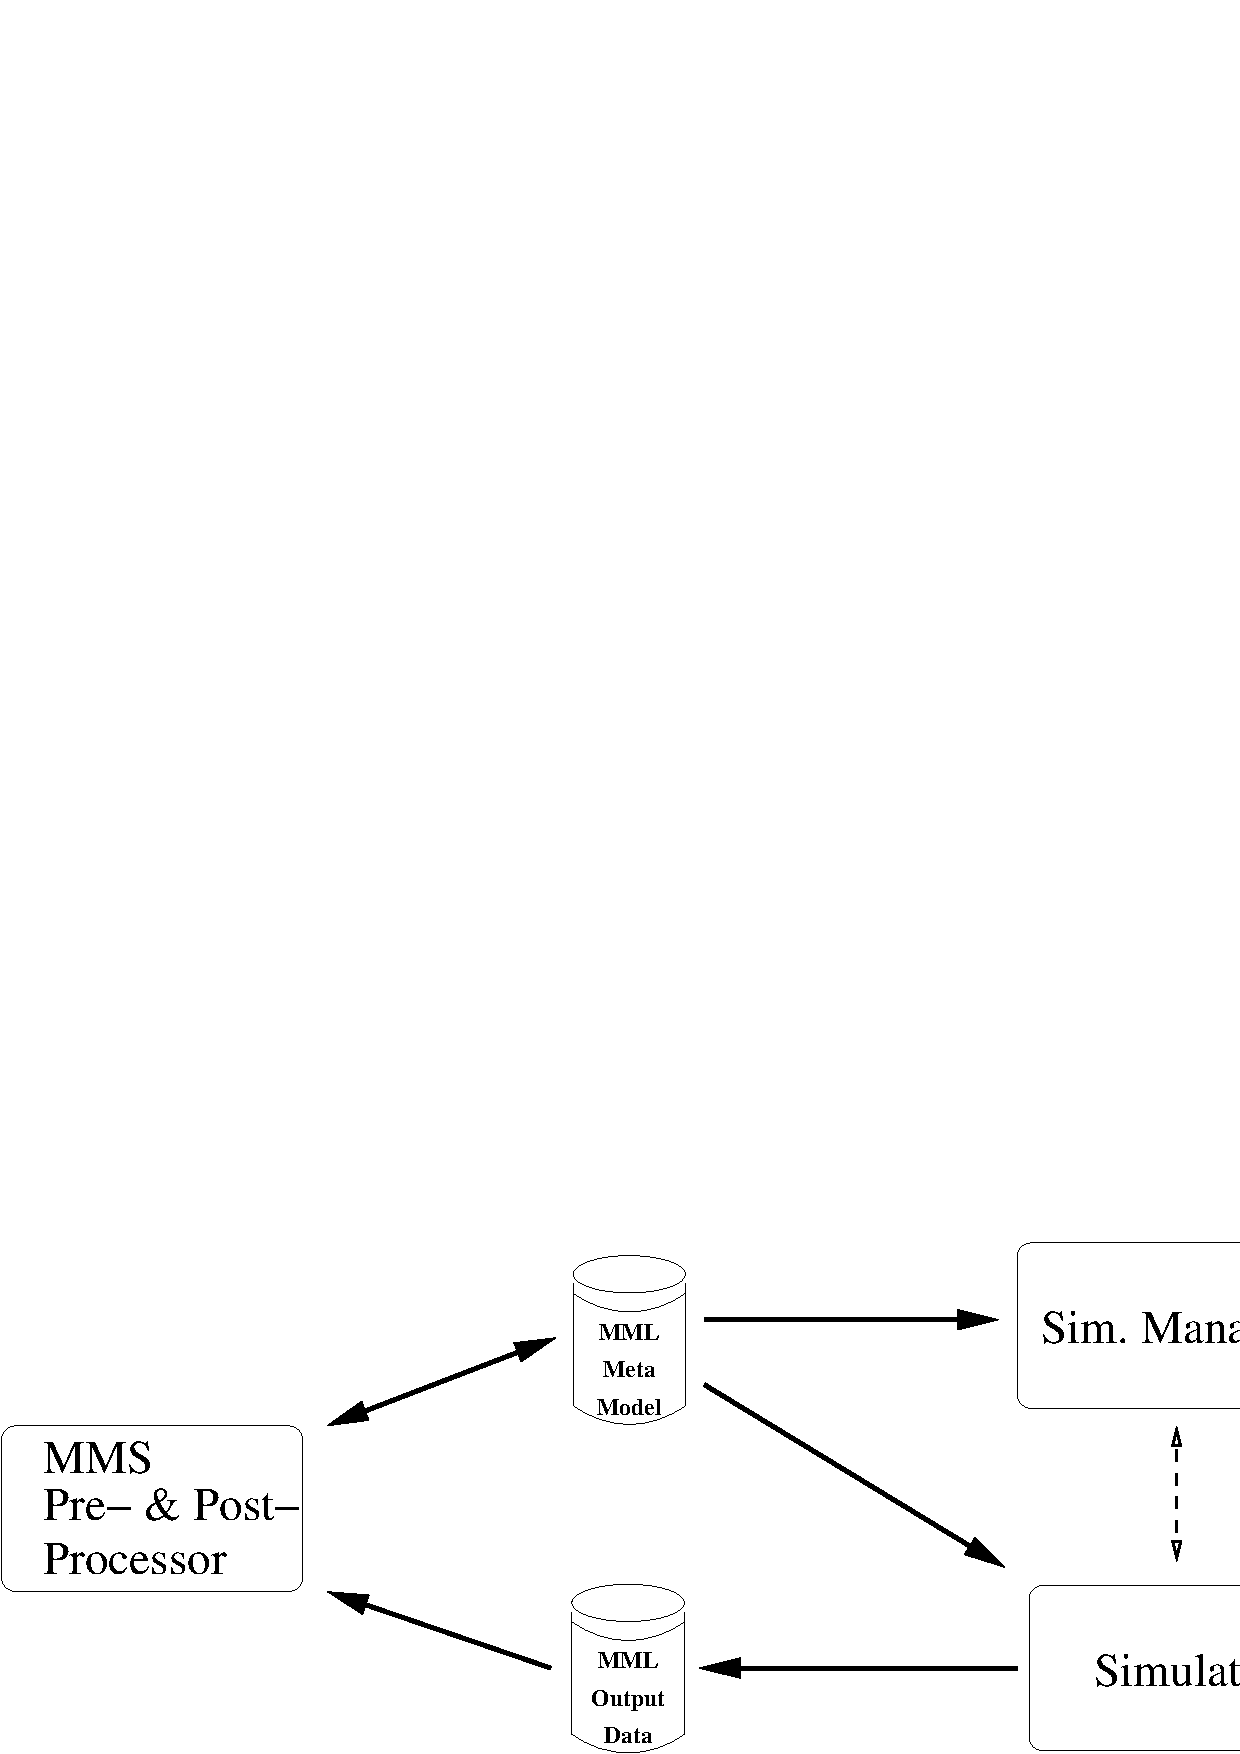
\includegraphics[width=9cm]{figs/MetaModelSysDesign2.pdf}}
    \caption{The system design for the meta-model simulation
    environment. } \label{fig:SystemDesign}
\end{center}\end{figure}

In addition to the {\em simulation manager} a meta-model {\em
  simulator} is included in the design that can start and monitor the
meta-model simulation.
%It creates its own internal meta-model
%structure for best simulation control and storage of meta-model
%simulation results.
The simulation manager has been designed to act as a network server
that allows several clients to connect and monitor the data flow
between the interconnected external model simulators. The {\em
  simulator} can connect to this port. All data received by the
simulation manager from the external model simulators is passed on to
the simulator that stores results in the meta-model output file.  This
client server architecture has some advantages over an integrated
solution where the simulation manager is part of the simulator:
\begin{itemize}
%\item Improved performance of the simulation manager because all file
%	I/O is handled by the simulator.
\item The simulator and simulation manager can run on different machines,
	this is useful, for instance, if the simulation start up must
	be performed on a machine other than the user's local machine.
\item Other processes can connect to the simulation manager's
	monitoring port. This allows, for instance, to visually
	monitor the co-simulation.
\end{itemize}

The simulation-manager manages start up of the different
simulation tools (external model simulators) and communication between
these tools, as defined by the simulation framework, see
Figure~\ref{fig:MMSystem}. Each simulation tool implements the
interface plug-in that handles the necessary communication with the
simulation manager. The manager keeps an internal interconnection
table for all connected external interfaces and forwards all received
packages accordingly.

\begin{figure}[ht]\begin{center}
%    \setlength{\unitlength}{0.00087489in}
%
\begingroup\makeatletter\ifx\SetFigFont\undefined%
\gdef\SetFigFont#1#2#3#4#5{%
  \reset@font\fontsize{#1}{#2pt}%
  \fontfamily{#3}\fontseries{#4}\fontshape{#5}%
  \selectfont}%
\fi\endgroup%
{\renewcommand{\dashlinestretch}{30}
\begin{picture}(6048,5823)(0,-10)
\put(1344.377,3582.324){\arc{1245.924}{0.4048}{2.8429}}
\blacken\path(797.429,3329.777)(749.000,3399.000)(759.156,3315.130)(797.429,3329.777)
\put(3584.161,4223.729){\arc{562.723}{4.6869}{8.1023}}
\blacken\path(3660.873,4515.131)(3577.000,4505.000)(3655.773,4474.470)(3660.873,4515.131)
\put(4175.044,3639.532){\arc{979.217}{0.6661}{2.8971}}
\blacken\path(4519.208,3263.018)(4560.000,3337.000)(4489.192,3290.918)(4519.208,3263.018)
\put(2163.567,5181.406){\arc{749.004}{1.7359}{4.8745}}
\blacken\path(2141.124,5534.604)(2224.000,5551.000)(2143.158,5575.533)(2141.124,5534.604)
\put(3570.744,5190.695){\arc{757.493}{4.3990}{7.8375}}
\blacken\path(3655.674,4842.785)(3577.000,4812.000)(3660.905,4802.141)(3655.674,4842.785)
\put(453.521,3379.929){\arc{4279.820}{0.0201}{1.0142}}
\blacken\path(1641.400,1624.988)(1584.000,1563.000)(1663.818,1590.683)(1641.400,1624.988)
\put(-793.797,1402.000){\arc{8528.231}{5.8122}{6.4064}}
\blacken\path(3426.420,961.685)(3438.000,878.000)(3467.163,957.289)(3426.420,961.685)
\put(5622.020,3483.229){\arc{4836.890}{2.1368}{3.0811}}
\blacken\path(4245.323,1470.087)(4325.000,1442.000)(4267.914,1504.277)(4245.323,1470.087)
\put(2034.068,735.905){\arc{748.181}{1.7375}{4.8760}}
\blacken\path(2012.101,1088.720)(2095.000,1105.000)(2014.193,1129.647)(2012.101,1088.720)
\put(3352.880,740.063){\arc{759.917}{4.7232}{7.5128}}
\blacken\path(3544.918,436.064)(3480.000,382.000)(3562.723,399.153)(3544.918,436.064)
\path(1856,3951)(3700,3951)(3700,3337)
	(1856,3337)(1856,3951)
\path(4560,3951)(6036,3951)(6036,3091)
	(4560,3091)(4560,3951)
\put(4805,4135){\arc{120}{1.5708}{3.1416}}
\put(4805,4507){\arc{120}{3.1416}{4.7124}}
\put(5791,4507){\arc{120}{4.7124}{6.2832}}
\put(5791,4135){\arc{120}{0}{1.5708}}
\path(4745,4135)(4745,4507)
\path(4805,4567)(5791,4567)
\path(5851,4507)(5851,4135)
\path(5791,4075)(4805,4075)
\path(2102,5120)(3577,5120)(3577,4259)
	(2102,4259)(2102,5120)
\path(2224,5796)(3454,5796)(3454,4874)
	(2224,4874)(2224,5796)
\put(2346,5302){\arc{120}{1.5708}{3.1416}}
\put(2346,5674){\arc{120}{3.1416}{4.7124}}
\put(3332,5674){\arc{120}{4.7124}{6.2832}}
\put(3332,5302){\arc{120}{0}{1.5708}}
\path(2286,5302)(2286,5674)
\path(2346,5734)(3332,5734)
\path(3392,5674)(3392,5302)
\path(3332,5242)(2346,5242)
\path(12,4259)(1487,4259)(1487,3399)
	(12,3399)(12,4259)
\path(135,4935)(1365,4935)(1365,4013)
	(135,4013)(135,4935)
\put(257,4442){\arc{120}{1.5708}{3.1416}}
\put(257,4814){\arc{120}{3.1416}{4.7124}}
\put(1243,4814){\arc{120}{4.7124}{6.2832}}
\put(1243,4442){\arc{120}{0}{1.5708}}
\path(197,4442)(197,4814)
\path(257,4874)(1243,4874)
\path(1303,4814)(1303,4442)
\path(1243,4382)(257,4382)
\blacken\path(1506.466,2401.443)(1463.000,2329.000)(1535.443,2372.466)(1506.466,2401.443)
\path(1463,2329)(2471,3337)
\blacken\path(2427.534,3264.557)(2471.000,3337.000)(2398.557,3293.534)(2427.534,3264.557)
\blacken\path(1380.074,4593.404)(1303.000,4628.000)(1354.726,4561.204)(1380.074,4593.404)
\path(1303,4628)(2163,3951)
\blacken\path(2085.926,3985.596)(2163.000,3951.000)(2111.274,4017.796)(2085.926,3985.596)
\blacken\path(3310.510,4032.960)(3331.000,3951.000)(3351.490,4032.960)(3310.510,4032.960)
\path(3331,3951)(3331,5242)
\blacken\path(3351.490,5160.040)(3331.000,5242.000)(3310.510,5160.040)(3351.490,5160.040)
\blacken\path(3757.646,3705.760)(3700.000,3644.000)(3779.927,3671.366)(3757.646,3705.760)
\path(3700,3644)(4745,4321)
\blacken\path(4687.354,4259.240)(4745.000,4321.000)(4665.073,4293.634)(4687.354,4259.240)
\blacken\path(4491.453,2366.813)(4567.000,2329.000)(4518.135,2397.917)(4491.453,2366.813)
\path(4567,2329)(3392,3337)
\blacken\path(3467.547,3299.187)(3392.000,3337.000)(3440.865,3268.083)(3467.547,3299.187)
\blacken\path(2727.379,1645.172)(2747.000,1563.000)(2768.356,1644.739)(2727.379,1645.172)
\path(2747,1563)(2766,3358)
\blacken\path(2785.621,3275.828)(2766.000,3358.000)(2744.644,3276.261)(2785.621,3275.828)
\path(4345,1658)(5820,1658)(5820,797)
	(4345,797)(4345,1658)
\path(4468,2334)(5697,2334)(5697,1412)
	(4468,1412)(4468,2334)
\put(4589,1841){\arc{120}{1.5708}{3.1416}}
\put(4589,2213){\arc{120}{3.1416}{4.7124}}
\put(5575,2213){\arc{120}{4.7124}{6.2832}}
\put(5575,1841){\arc{120}{0}{1.5708}}
\path(4529,1841)(4529,2213)
\path(4589,2273)(5575,2273)
\path(5635,2213)(5635,1841)
\path(5575,1781)(4589,1781)
\path(4683,4648)(5913,4648)(5913,3726)
	(4683,3726)(4683,4648)
\path(128,1921)(1603,1921)(1603,1061)
	(128,1061)(128,1921)
\path(251,2597)(1480,2597)(1480,1675)
	(251,1675)(251,2597)
\put(372,2104){\arc{120}{1.5708}{3.1416}}
\put(372,2476){\arc{120}{3.1416}{4.7124}}
\put(1358,2476){\arc{120}{4.7124}{6.2832}}
\put(1358,2104){\arc{120}{0}{1.5708}}
\path(312,2104)(312,2476)
\path(372,2536)(1358,2536)
\path(1418,2476)(1418,2104)
\path(1358,2044)(372,2044)
\path(1982,872)(3457,872)(3457,12)
	(1982,12)(1982,872)
\path(2105,1549)(3334,1549)(3334,627)
	(2105,627)(2105,1549)
\put(2226,1056){\arc{120}{1.5708}{3.1416}}
\put(2226,1428){\arc{120}{3.1416}{4.7124}}
\put(3212,1428){\arc{120}{4.7124}{6.2832}}
\put(3212,1056){\arc{120}{0}{1.5708}}
\path(2166,1056)(2166,1428)
\path(2226,1488)(3212,1488)
\path(3272,1428)(3272,1056)
\path(3212,996)(2226,996)
\put(2471,3583){\makebox(0,0)[lb]{{\SetFigFont{8}{9.6}{\rmdefault}{\mddefault}{\updefault}Sim. Manager}}}
\put(4253,3337){\makebox(0,0)[lb]{{\SetFigFont{8}{9.6}{\rmdefault}{\mddefault}{\updefault}\emph{Start}}}}
\put(381,3214){\makebox(0,0)[lb]{{\SetFigFont{8}{9.6}{\rmdefault}{\mddefault}{\updefault}\emph{Start}}}}
\put(5114,3337){\makebox(0,0)[lb]{{\SetFigFont{8}{9.6}{\rmdefault}{\mddefault}{\updefault}Simulink}}}
\put(2655,4505){\makebox(0,0)[lb]{{\SetFigFont{8}{9.6}{\rmdefault}{\mddefault}{\updefault}Modelica}}}
\put(381,3644){\makebox(0,0)[lb]{{\SetFigFont{8}{9.6}{\rmdefault}{\mddefault}{\updefault}MSC.ADAMS}}}
\put(3823,4505){\makebox(0,0)[lb]{{\SetFigFont{8}{9.6}{\rmdefault}{\mddefault}{\updefault}\emph{Start}}}}
\put(1487,4505){\makebox(0,0)[lb]{{\SetFigFont{8}{9.6}{\rmdefault}{\mddefault}{\updefault} TLM data}}}
\put(2840,4075){\makebox(0,0)[lb]{{\SetFigFont{8}{9.6}{\rmdefault}{\mddefault}{\updefault} TLM data}}}
\put(3884,3706){\makebox(0,0)[lb]{{\SetFigFont{8}{9.6}{\rmdefault}{\mddefault}{\updefault} TLM data}}}
\put(1303,5242){\makebox(0,0)[lb]{{\SetFigFont{8}{9.6}{\rmdefault}{\mddefault}{\updefault}\parbox{10cm}{time step,\newline position,\newline velocity}}}}
\put(3700,4751){\makebox(0,0)[lb]{{\SetFigFont{8}{9.6}{\rmdefault}{\mddefault}{\updefault}Force, torque}}}
\put(4244,2692){\makebox(0,0)[lb]{{\SetFigFont{8}{9.6}{\rmdefault}{\mddefault}{\updefault} TLM data}}}
\put(1785,2571){\makebox(0,0)[lb]{{\SetFigFont{8}{9.6}{\rmdefault}{\mddefault}{\updefault} TLM data}}}
\put(3680,2128){\makebox(0,0)[lb]{{\SetFigFont{8}{9.6}{\rmdefault}{\mddefault}{\updefault}\emph{Start}}}}
\put(1987,2248){\makebox(0,0)[lb]{{\SetFigFont{8}{9.6}{\rmdefault}{\mddefault}{\updefault}\emph{Start}}}}
\put(3519,1603){\makebox(0,0)[lb]{{\SetFigFont{8}{9.6}{\rmdefault}{\mddefault}{\updefault}\emph{Start}}}}
\put(2753,2208){\makebox(0,0)[lb]{{\SetFigFont{8}{9.6}{\rmdefault}{\mddefault}{\updefault} TLM data}}}
\put(3761,515){\makebox(0,0)[lb]{{\SetFigFont{8}{9.6}{\rmdefault}{\mddefault}{\updefault}Force, torque}}}
\put(1100,354){\makebox(0,0)[lb]{{\SetFigFont{8}{9.6}{\rmdefault}{\mddefault}{\updefault}\parbox{5cm}{time step,\newline position,\newline velocity}}}}
\put(4898,1044){\makebox(0,0)[lb]{{\SetFigFont{8}{9.6}{\rmdefault}{\mddefault}{\updefault}Orpheus}}}
\put(2352,5481){\makebox(0,0)[lb]{{\SetFigFont{8}{9.6}{\rmdefault}{\mddefault}{\updefault}Interface plugin}}}
\put(237,4581){\makebox(0,0)[lb]{{\SetFigFont{8}{9.6}{\rmdefault}{\mddefault}{\updefault}Interface plugin}}}
\put(4602,1971){\makebox(0,0)[lb]{{\SetFigFont{8}{9.6}{\rmdefault}{\mddefault}{\updefault}Interface plugin}}}
\put(4782,4266){\makebox(0,0)[lb]{{\SetFigFont{8}{9.6}{\rmdefault}{\mddefault}{\updefault}Interface plugin}}}
\put(4782,3771){\makebox(0,0)[lb]{{\SetFigFont{8}{9.6}{\rmdefault}{\mddefault}{\updefault}Plugin wrapper}}}
\put(681,1306){\makebox(0,0)[lb]{{\SetFigFont{8}{9.6}{\rmdefault}{\mddefault}{\updefault}BEAST}}}
\put(2535,258){\makebox(0,0)[lb]{{\SetFigFont{8}{9.6}{\rmdefault}{\mddefault}{\updefault}BEAST}}}
\put(2217,1206){\makebox(0,0)[lb]{{\SetFigFont{8}{9.6}{\rmdefault}{\mddefault}{\updefault}Interface plugin}}}
\put(372,2241){\makebox(0,0)[lb]{{\SetFigFont{8}{9.6}{\rmdefault}{\mddefault}{\updefault}Interface plugin}}}
\put(417,1746){\makebox(0,0)[lb]{{\SetFigFont{8}{9.6}{\rmdefault}{\mddefault}{\updefault}Plugin wrapper}}}
\put(2217,711){\makebox(0,0)[lb]{{\SetFigFont{8}{9.6}{\rmdefault}{\mddefault}{\updefault}Plugin wrapper}}}
\put(4557,1476){\makebox(0,0)[lb]{{\SetFigFont{8}{9.6}{\rmdefault}{\mddefault}{\updefault}Plugin wrapper}}}
\put(2307,4941){\makebox(0,0)[lb]{{\SetFigFont{8}{9.6}{\rmdefault}{\mddefault}{\updefault}Plugin wrapper}}}
\put(237,4086){\makebox(0,0)[lb]{{\SetFigFont{8}{9.6}{\rmdefault}{\mddefault}{\updefault}Plugin wrapper}}}
\end{picture}
}

   {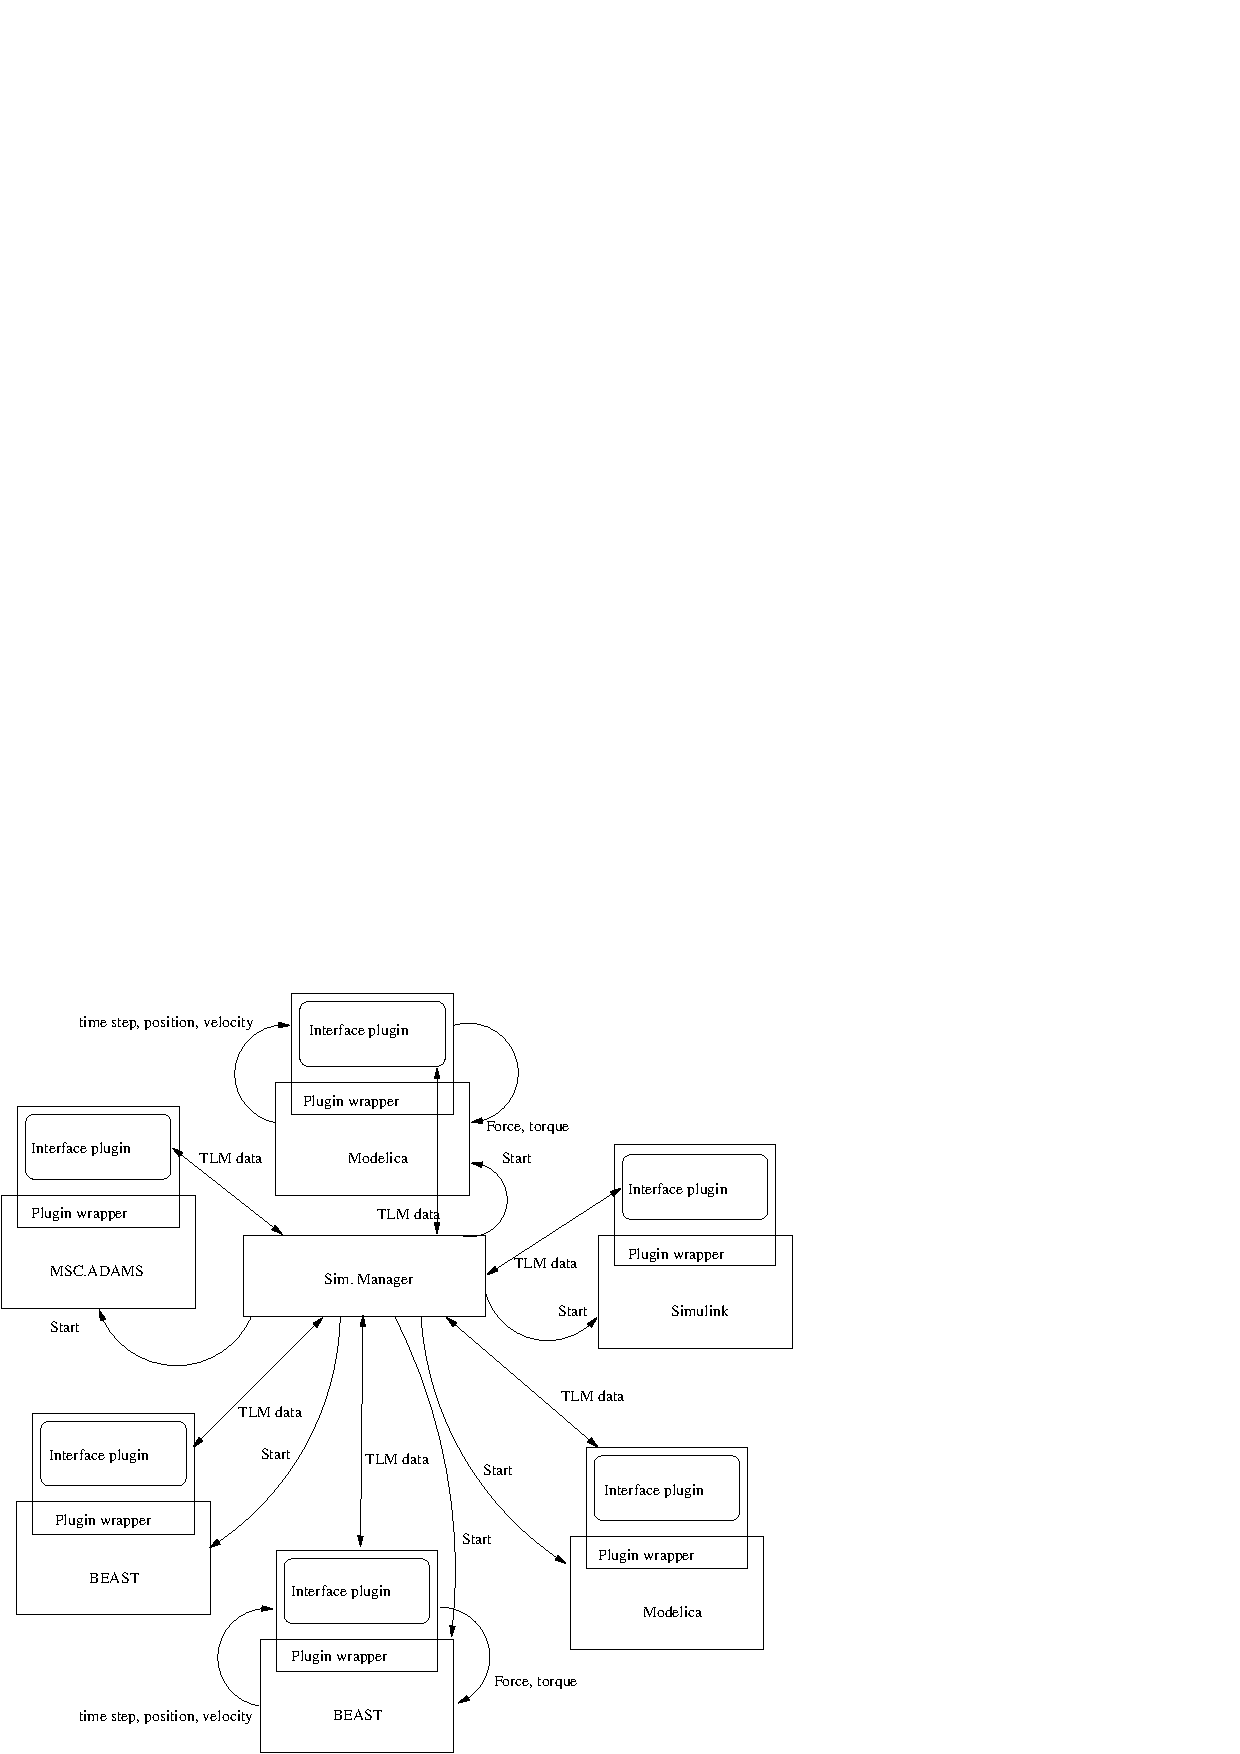
\includegraphics[width=9cm]{figs/TLM_system.pdf}}
    \caption{The simulation manager handles start up and communication
	between the tool specific simulators.}
    \label{fig:MMSystem}
\end{center}\end{figure}

Simulation results can be analysed in the post-processing
applications, i.e., a two dimensional plotting program and a three
dimensional visualisation tool, i.e., the meta-model editor
(MME). Data animation of system dynamics is possible to a limited
extent based on the data that is exchanged in the external interfaces.

\section{Meta-Model XML Files}
\label{meta}
The TLM default implementation contains a XML meta-model reader, that
can be used by the simulation manager to read the meta-model from an
XML file.

A Meta-Model contains the following XML nodes:
\begin{description}
\item[Model] is the top Meta-Model node that contains a list of {\tt SubModels} and {\tt Connections}.
\item[SubModels] is the node that contains the list of all {\tt SubModel} nodes.
\item[SubModel] is used for the external models. There is a {\tt
  SubModel} node for each external model that participates in the
  co-simulation. It defines a sub-model name used in the meta-model
  and the start method and the simulation tool specific model files
  that needed to run the simulation. Each {\tt SubModel} node also
  contains a list of {\tt InterfacePoint} nodes.
\item[InterfacePoint] nodes are used to specify the TLM interfaces of
  each external model, that is, each {\tt SubModel}. It defines the
  name of a certain interface in the external model.
\item[Connections] is the node that contains the list of all {\tt Connection} nodes.
\item[Connection] nodes define connections between two connected {\tt
  InterfacePoint}s, that is, a connection between two TLM
  interfaces. TLM parameters are specified for each connection.
\item[SimulationParams] node defines global meta-model simulation
  parameters. Total simulation start time, end time, and network port
  are defined in this node.
\end{description}


Here a sample meta-model XML file for a Modelica with Beast co-simulation:
{\scriptsize
\begin{verbatim}
<?xml version="1.0" encoding="ISO-8859-1"?>

<!-- The root node is the meta-model -->
<Model Name="Pendulum">

    <!-- List of connected sub-models -->
    <SubModels>	

        <SubModel Name="shaft1"
                StartCommand="StartTLMModelica"
                ExactStep="0"
                ModelFile="shaft1.mo">

                <!-- TLM interface points for SubModel A -->
                <InterfacePoint Name="tlm"/>
        </SubModel>

        <SubModel Name="brg1"
                StartCommand="StartTLMBeast"
                ExactStep="0"
                ModelFile="dgbb">

                <!-- TLM interface points for SubModel C -->
                <InterfacePoint Name="bIR`cs1"/>
                <InterfacePoint Name="bER`cs1"/>
        </SubModel>

        <SubModel Name="shaft2"
                StartCommand="StartTLMModelica"
                ExactStep="0"
                ModelFile="shaft2.mo">

                <!-- TLM interface points for SubModel C -->
                <InterfacePoint Name="tlm"/>
        </SubModel>

    </SubModels>

    <!-- List of TLM connections -->
    <Connections>
	<!-- Some more physical values: Delay="1e-5" Zf="8e4" Zfr="400" alpha="0.2" -->
        <Connection From="shaft1.tlm" To="brg1.bER`cs1"
		Delay="1e-3" Zf="1e4" Zfr="1e2" alpha="0.2"/>
        <Connection From="shaft2.tlm" To="brg1.bIR`cs1"
		Delay="1e-3" Zf="1e4" Zfr="1e2" alpha="0.2"/>
    </Connections>

    <!-- Parameters for the simulation -->
    <SimulationParams ManagerPort="11113"
                StartTime="0"
                StopTime="1"
                NetworkTimeout="600"/>

</Model>
\end{verbatim}
}

\chapter{TLM background theory}
\label{secTLMtheory}
The method that is used to enable interaction between dynamic models in the composite model simulation is \emph{transmission line modelling} (TLM)~\cite{Johns-80}~\cite{KrusModMech-99}~\cite{KrusDistrSim}~\cite{Cogan-06}.
TLM uses physically motivated time delays to separate the components in time and enable efficient co-simulation. 
Only TLM connections between two external interfaces are currently supported by the composite model simulation environment because the TLM method gives numerical stability.


The TLM (\emph{Transmission Line Modeling}) method, also called Bilateral Delay Line Method \cite{Johns-80}, exploites the fact that all physical interactions in nature have finite propagation speed.
\begin{figure}
\begin{center}
   {\includegraphics[width=9cm]{figs/TLMline.png}}
\caption{Delay line with the passing wave variables $c_1$ and $c_2$
and velocity variables $v_1$ and $v_2$.}
\end{center}
\label{figTLMline}
\end{figure}

A basic one-dimensional transmission line is shown in Figure \ref{figTLMline}.
For the mechanical case the line is basically an ideal elastic medium with force waves $c_1$ and $c_2$ going between its ends. 
The input disturbances are velocities $v_1$ and $v_2$ and the forces from the transmission line $F_1$ and $F_2$.

Note that the springs in our implementation are assumed to be isotropic.
That is no cross-term waves are generated when working in 2D and 3D. 
See \cite{KrusModMech-99} for further discussions.

If the line delay is set to $T_{TLM}$ and its impedance to $Z_F$ then the govering equations are:
\begin{equation}
\begin{array}{l}
c_1(t) = F_2(t-T_{TLM})+ Z_F \; v_2(t-T_{TLM})\\
c_2(t) = F_1(t-T_{TLM})+ Z_F \; v_1(t-T_{TLM})\\
\\
F_1(t) = Z_F \; v_1(t) + c_1(t) \\
F_2(t) = Z_F \; v_2(t) + c_2(t)
\end{array}
\label{eqTLM}
\end{equation}
The equations show that the two simulation systems are decoupled with the delay time $T_{TLM}$. Simulation framework can utilize this decoupling to enable efficient communications during co-simulation. 

Representing the TLM connection with a simple model of a steel beam, the stiffness coefficient can be computed as (see \cite{KrusModMech-99}):
\begin{equation}
\label{eqKsimple}
k = \frac{E A}{L_0}
\end{equation}
where $E$ is Young's modulus, $A$ is the cross section area and $L_0$ the length of the beam. 

The impedance $Z_F$ has a relation to the spring constant $k$, $Z_F = k T_{TLM}$. 
The impedance factor can then be formulated as a function of the area and length of the steel rod according to
\begin{equation}
\label{eqZFsimple}
Z_F = \frac{E A T_{TLM}}{L_0}
\end{equation}

\begin{figure}
\begin{center}
   {\includegraphics[width=9cm]{figs/RotStiff.png}}
\caption{Estimating the rotational stiffness.}
\end{center}
\label{figRotStiff}
\end{figure}

To get the stiffness and impedance for the rotational degrees of freedom one can use the already computed stiffness $k$. If the arrangement depicted in
Figure \ref{figRotStiff} is assumed, then:
\begin{equation}
k_{\phi} = \frac{M}{\delta_{\phi}} = 2 \frac{ (k/2) \delta_{\phi} (L_0/2)^2}{\delta_{\phi}} = \frac{k L_0^2}{4}
\label{eqKphi}
\end{equation}

and the impedance for the rotation:
\begin{equation}
Z_{FR} = \frac{1}{4}Z_F L_0^2
\end{equation}

The time constant $T_{TLM}$ can be computed using the speed of sound for the medium:
\begin{equation}
\label{eqTtlm}
T_{TLM} = \frac{L_0}{v_{medium}}
\end{equation}

It can be shown that the TLM element also introduces a (\emph{parasitic mass}) that can be viewed to be outside the simulated system \cite{KrusModMech-99}. The total mass for the combined systems must therefore also
include the parasitic mass of the TLM element in order to make, e.g., the energy conservation formulas correct. This mass depends on the impedance factor and the time delay factor
\begin{equation}
\label{eqMtlm}
m_p = Z_F T_{TLM}
\end{equation}

This implies that if the impedance factor $Z_F$  is increased, the parasitic mass will increase if the synchronization delay $T_{TLM}$ is not decreased. 
If the parasitic mass is large it may influence the system behavior and can not be neglected. 
Note, that for the simple beam case when TLM parameters are computed according to Equations \ref{eqZFsimple} and \ref{eqTtlm} the parasitic mass is equivalent to the mass of the beam ($\rho A L0$, where $\rho$ is the material density).

For practical purposes (see \cite{Fritzson+Stahl+Nakhimovski-07}) one can use the parameters of a material cube with an edge given by \emph{characteristic distance} $L_0$. 
Equations \ref{eqKsimple} and \ref{eqKphi} can then be used to compute the translational and rotational stiffnesses:
\begin{equation}
\begin{array}{l}
k = \frac{E L_0 ^2}{L_0} = E L_0 \\
\\
k_{\phi} = \frac{k L_0^2}{4} = \frac{E L_0^3}{4}
\end{array}
\end{equation}

To give a concrete example, let us assume that connection medium is steel and the characteristic length is $L_0 = 0.1$. Steel has  Young's modulus $E = 210 GPa$ and the speed of sound in steel is $v_{steel}=5180 m/s$.
The TLM parameters then can be computed:
\begin{equation}
\begin{array}{l}
T_{TLM} = L_0 / v_{steel} \approx 2*10^{-5} \\
\\
Z_F =  E L_0 T_{TLM} \approx 2 * 10^5 \\
\\
Z_{FR} =  \frac{1}{4}Z_F L_0^2 \approx 500
\end{array}
\end{equation}

Calculations like these give approximate values of the stiffness and the time delay of the TLM element. 
This gives a background for selecting the TLM line delay and impedance parameters.
In cases when required $T_{TLM}$ becomes a limiting factor, while the TLM link stiffness is much higher than the stiffnesses used in the sub-models, a lower stiffness and larger $T_{TLM}$ may be considered.

The elastic medium that is modelled with the TLM element introduces oscillation frequencies (standing waves) given by:
\begin{equation}
\label{eqTspring}
f_{TLM, i} = \frac{i}{2\;T_{TLM}}, \;\; i = 1, 2, 3, ...
\end{equation}

The basic TLM model has no damping which can result in unwanted vibrations during simulation.
In \cite{KrusModMech-99} a low pass filtering of the TLM charateristics is recommended:
\begin{equation}
c_{\ri{filtered}}(t) = c_{\ri{filtered}}(t - T) \; \alpha + c(t) \; (1 - \alpha)
\end{equation}
The filtering is controlled by a damping constant $\alpha$. 
The recommended value according to~ \cite{KrusModMech-99} is $0.2$.



%\chapter{Design and Implementation}
\chapter{TLMManager System Design}
The TLMManager is responsible for managing the TLM based co-simulation. 
The main component used in the TLMManager is an instance of {\em ManagerCommHandler} that takes a composite model as input.
{\scriptsize
\begin{verbatim}
    //! Constructor.
    ManagerCommHandler(MetaModel& Model):
        MessageQueue(),
        Comm(Model.GetComponentsNum(), Model.GetSimParams().GetPort()),
        TheModel(Model),
        CommMode(CoSimulationMode),
        monitorInterfaceMap(),
        monitorMapLock(),
        runningMode(StartUpMode)
    {
    };
\end{verbatim}
}

A {\em MetaModel} instance can be generated in different ways. 
The default TLM co-simulation implementation contains an XML composite model reader, see also Figure~\ref{fig:MetaModelReader}. 
For details about the XML composite model description see Section~\ref{meta}.

\begin{figure}[ht]
\begin{center}
  {\includegraphics[width=4cm]{figs/classMetaModelReader__coll__graph.png}}
\end{center}
\caption{UML collaboration diagram of the MetaModelReader class. The
  MetaModel reader initialized the MetaModel data structure.}
\label{fig:MetaModelReader}
\end{figure}

The {\em MetaModelReader} parses the XML composite model file and initializes {\em MetaModel} and {\em SimulationParams} data structures, that is, set-up co-simulation parameters. 
Simulation parameters define global co-simulation settings, e.g., start and end time. 
Composite model parameters define the co-simulation components (simulation models) and their interconnection.

The {\em ManagerCommHandler} is then started, that is, the {\em Run()} function is invoked. 
This function initialized the different threads that are used during the co-simulation:
{\scriptsize
\begin{verbatim}
// Run method executes all the protocols in the right order:
// Startup, Check then Simulate
void ManagerCommHandler::Run(CommunicationMode CommMode_In) {
    CommMode = CommMode_In;

    pthread_attr_t attr;
    pthread_attr_init(&attr);
    pthread_attr_setscope(&attr,  PTHREAD_SCOPE_SYSTEM);
    pthread_t reader, writer;

    // start the reader & writer threads
    pthread_create( &reader, &attr, thread_ReaderThreadRun, (void*)this);

    pthread_create( &writer, &attr, thread_WriterThreadRun, (void*)this);

    // Start the minitoring thread
    pthread_t monitor;
    if( CommMode == CoSimulationMode ){
        pthread_create( &monitor, &attr, thread_MonitorThreadRun, (void*)this);
    }

    // Wait until all threads are finished.
    pthread_join(reader, NULL);
    pthread_join(writer, NULL);

    if( CommMode == CoSimulationMode ){
        pthread_join(monitor, NULL);
    }
}
\end{verbatim}
}

Note, that all communication between the co-simulation participants (simulators with models) is going through the TLM manager. 
This communication is handled by the threads that are started in the {\em Run()} function. 
The following threads are started:
\begin{description}
\item[The reader thread] initialized the co-simulation, processes incoming messages, and creates messages to be sent. 
This threads first task is to run the {\em RunStartupProtocol()} that starts all the simulation tools that are participating in the co-simulation and runs the initiation protocol. 
After that the thread goes into message passing mode. 
Messages from one co-simulation participant to another are taken by the reader thread and marshaled to the receiver, that is, they are converted into outgoing messages.
\item[The writer thread] processes all outgoing messages. 
It loops through the queue of outgoing messages and distributes them to the correct receivers.
\item[The monitor thread] copies and forwards all outgoing messages to any connected monitoring process. 
This can be used to monitor the co-simulation. 
If no monitoring process is connected no copying and forwarding will take place.
\end{description}

\begin{figure}
    \begin{center}
    \includegraphics[width=9cm]{figs/classManagerCommHandler__coll__graph.png}
      \caption{ManagerCommHandler collaboration and class diagram.}
      \label{fig:ManagerCommHandlerClassDesign}
    \end{center}
\end{figure}

The {\em ManagerCommHandler} collaborates with different classes to handle co-simulation start-up and communication, see also Figure~\ref{fig:ManagerCommHandlerClassDesign}. 
{\em TLMManagerComm} is responsible for all socket communications on the TLMManager side. The {\em TLMMessageQueue} handles the queue for outgoing messages.

\subsection{Co-Simulation Start-up}
During co-simulation start-up the TLMManager starts the different co-simulation components (external models) and then waits until all components have registered themselves. 
This is done with a simple initialization protocol.

First the components are started using {\tt TLMComponentProxy::StartComponent(...)}. 
This is done using the OS specific execution method, for instance, with {\it fork()} and {\it execlp(...)} on Linux:
{\scriptsize
\begin{verbatim}
  execlp( StartCommand.c_str(), StartCommand.c_str(),
          Name.c_str(),
          startTime.c_str(),
          endTime.c_str(),
          strMaxStep.c_str(),
          serverName.c_str(),
          ModelName.c_str(),
          NULL );
\end{verbatim}
}

The start command is the start-up script that must be provided for each specific simulation tool. 
It takes a couple of parameters as specified in the composite model XML file:
\begin{description}
\item[Name] of the component as specified in the composite model XML file.
\item[Start time] of the simulation in seconds, typically 0.
\item[End time] of the simulation in seconds.
\item[Max step] for the solver to take. This is a limit set by the TLM interfaces of the specific component. 
The solver is not allowed to take larger steps.
\item[Server name] is typically the hostname or IP address that the TLMManager is running on and the port number that it is using. 
For  instance {\it 163.157.1.23:1111}.
\item[Model name] of the simulation model. Typically the input file
  needed to start the external model simulation.
\end{description}

\subsection{External Model Initialization}
After external model start-up, the TLMManager waits until all external models have registered themselves. 
This is performed in {\em ManagerCommHandler::RunStartupProtocol()}. 
Here an outline of the code:
{\scriptsize
\begin{verbatim}
void ManagerCommHandler::RunStartupProtocol() {
    ...
    // Start the external components forming "coupled simulation"
    TheModel.StartComponents();

    // Setup timer
    tTM_Info tInfo;
    TM_Init(&tInfo);
    TM_Start(&tInfo);

    while( (numToRegister > 0) ||
           ( numCheckModel < TheModel.GetComponentsNum()) ) {
        ...

        // Check all the registered components if they send
        // interface registration messages.
        for(int iSock =  TheModel.GetComponentsNum() - 1; iSock >= 0 ; --iSock) {
            ...
            TLMMessage* message = MessageQueue.GetReadSlot();
            message->SocketHandle = hdl;
            TLMCommUtil::ReceiveMessage(*message);

            if(message->Header.MessageType == TLMMessageTypeConst::TLM_CHECK_MODEL) {
                // This component is done with registration. It's will wait for others
                TLMErrorLog::Log(string("Component ") + comp.GetName() + " is ready to simulation");;

                comp.SetReadyToSim();
                numCheckModel++;
            }
            else {
                TLMErrorLog::Log(string("Component ") + comp.GetName() + " registers interface");;

                Comm.AddActiveSocket(hdl); // expect more messages
                ProcessRegInterfaceMessage(iSock, *message);
                MessageQueue.PutWriteSlot(message);
            }
        }

        // Check if a new connection is waiting to be accepted.
        if((numToRegister > 0) && Comm.HasData(acceptSocket)) {
            int hdl = Comm.AcceptComponentConnections();
            TLMMessage* message = MessageQueue.GetReadSlot();
            message->SocketHandle = hdl;

            if( !TLMCommUtil::ReceiveMessage(*message) ){
                TLMErrorLog::FatalError("Failed to get message, exiting");
                abort();
            }

            ProcessRegComponentMessage(*message);

            MessageQueue.PutWriteSlot(message);
            numToRegister --;
            if(numToRegister == 0)
                TLMErrorLog::Log("All expected components are registered");

            Comm.AddActiveSocket(hdl);
        }

        if(numToRegister)  // still more connections expected
            Comm.AddActiveSocket(acceptSocket);

    }
}
\end{verbatim}
}
The above method has two main tasks, first to check for new connections from any external model. 
Second to check if already registered components need to register any TLM interfaces.

The initialization protocol looks the following way:
\begin{enumerate}
\item An external model send a TLMMessageTypeConst::TLM\_REG\_COMPONENT message to the TLMManager.
\item The TLMManager answers with the same message but also sets the data size of the message to 0.
\item The external model send an interface registration message (TLMMessageTypeConst::TLM\_REG\_INTERFACE).
\item The manager answers with the same message head and adds the connection parameters as stored in the composite model XML file to the data section of the message.
\item The external model repeats the interface registration for all its external (TLM) interfaces.
\item Finally the external model sends a TLMMessageTypeConst::TLM\_CHECK\_MODEL that tells that it is ready to simulate.
\item The TLMManager puts the component into {\em ready for simulation} mode.
\end{enumerate}


\chapter{Simulink TLM Plugin}

The Matlab/Simulink TLMPlugin implementation is based on a Matlab S-function interface.
There are blocks for 3D force interfaces, 1D signal input interfaces and 1D signal output interfaces.

{\scriptsize
\begin{verbatim}
/*
 * tlmforce.c: Based on 'C' template for a level 2 S-function.
 *
 *  -------------------------------------------------------------------------
 *  | See matlabroot/simulink/src/sfuntmpl_doc.c for a more detailed template |
 *  -------------------------------------------------------------------------
 *
 * Copyright 1990-2000 The MathWorks, Inc.
 * $Revision$
 */
\end{verbatim}
}

\noindent TLM delay is set in the initialization of the S-Function interface function {\em mdlInitializeSampleTimes(...).}

{\scriptsize
\begin{verbatim}
/* Function: mdlInitializeSampleTimes =========================================
 * Abstract:
 *    This function is used to specify the sample time(s) for your
 *    S-function. You must register the same number of sample times as
 *    specified in ssSetNumSampleTimes.
 */
static void mdlInitializeSampleTimes(SimStruct *S)
{
    double sTime, eTime, timeStep;
    TLM_InterfaceReg::GetInstance(false)->GetSimParameters(sTime, eTime, timeStep);
    // true or false in GetInstance(...) enables/disables debug output

    TLMErrorLog::Log("Set sample time to " + ToStr(timeStep));

    /* Set TLM delay here! */
    ssSetSampleTime(S, 0, CONTINUOUS_SAMPLE_TIME);
    ssSetOffsetTime(S, 0, 0.0);

    /* Set TLM delay here! */
    ssSetSampleTime(S, 1, timeStep);
    ssSetOffsetTime(S, 1, 0.0);
}
\end{verbatim}
}

\noindent Note, that the first call to {\em TLM\_InterfaceReg::GetInstance(...)} initialized the TLM plugin, that is, it reads the TLM configuration parameters form the config file.

Communication with Simulink is based on the C structure {\em SimStruct}. 
Initially we need to setup the size (of the data that we want to communicate in the structure. 
This is done in the S-Function interface function {\em mdlInitializeSizes(...)}.

{\scriptsize
\begin{verbatim}
/* Function: mdlInitializeSizes ===============================================
 * Abstract:
 *    The sizes information is used by Simulink to determine the S-function
 *    block's characteristics (number of inputs, outputs, states, etc.).
 */
static void mdlInitializeSizes(SimStruct *S)
{
    /* See sfuntmpl_doc.c for more details on the macros below */

    ...

    /* input ports are: */
    /* position[3]      Interface position data */
    /* orientation[3x3] Interface rotation matrix */
    /* speed[3]         Interface translational velocity */
    /* ang_speed[3]     Interface angular velocity */

    if (!ssSetNumInputPorts(S, 4)) return;
    /* Set size of input arrays */
    ssSetInputPortWidth(S, 0, 3);
    ssSetInputPortWidth(S, 1, 9);
    ssSetInputPortWidth(S, 2, 3);
    ssSetInputPortWidth(S, 3, 3);

    ...

    /* output ports are: */
    /* force[3]  Output force */
    /* moment[3] Output moment */

    if (!ssSetNumOutputPorts(S, 4)) return;
    ssSetOutputPortWidth(S, 0, 3);
    ssSetOutputPortWidth(S, 1, 3);
    ssSetOutputPortWidth(S, 2, 3);
    ssSetOutputPortWidth(S, 3, 9);

}
\end{verbatim}
}

\noindent The force calculation in the TLM interface takes place in the S-Function interface function {\em mdlOutputs(...)}. 
This function is called by Simuink for a given time instance. 
The motion of the interface can be extracted from the {\em SimStruct} structure that has been setup before, see {\em mdlInitializeSizes} above. 
The resulting load (force and moment) is stored in the same structure.

{\scriptsize
\begin{verbatim}
/* Function: mdlOutputs =======================================================
 * Abstract:
 *    In this function, you compute the outputs of your S-function
 *    block. Generally outputs are placed in the output vector, ssGetY(S).
 */
static void mdlOutputs(SimStruct *S, int_T tid)
{
    /* inputs: */
    /* position[3]      Interface position data */
    /* orientation[3x3] Interface rotation matrix */
    /* speed[3]         Interface translational velocity */
    /* ang_speed[3]     Interface angular velocity */
    double *R = (double*)ssGetInputPortSignal(S,0);
    double *A = (double*)ssGetInputPortSignal(S,1);
    double *vR = (double*)ssGetInputPortSignal(S,2);
    double *Omega = (double*)ssGetInputPortSignal(S,3);

    const char* name = ssGetPath(S);
    real_T time = ssGetT(S);

    int ifID = TLM_InterfaceReg::GetInstance()->GetInterfaceID(name);

    /* output */
    double force[6];
    TLMTimeData3D CurTimeData;

    if( ifID >= 0 ) {
        TLM_InterfaceReg::GetInstance()->GetPlugin()->GetForce3D(ifID,
                                                                 time,
                                                                 R,
                                                                 A,
                                                                 vR,
                                                                 Omega,
                                                                 force);

        /* Get Position and Orientation */
        TLM_InterfaceReg::GetInstance()->GetPlugin()->GetTimeData3D(ifID,
                                                                    time,
                                                                    CurTimeData);

    }
    else {
        /* Not connected */
        for( int i=0 ; i<6 ; i++ ) {
            force[i] = 0.0;
        }
    }

    /* ------- store the result ------- */

    /* Force & Moment */
    real_T  *f = ssGetOutputPortRealSignal(S,0);
    real_T  *m = ssGetOutputPortRealSignal(S,1);

    for( int i=0 ; i<3 ; i++ ){
        f[i] = force[i];
        m[i] = force[i+3];
    }

    /* Position & Orientation */
    real_T  *R_TLM = ssGetOutputPortRealSignal(S,2);
    real_T  *A_TLM = ssGetOutputPortRealSignal(S,3);

    for( int i=0 ; i<3 ; i++ ){
        R_TLM[i] = CurTimeData.Position[i];
        A_TLM[i] = CurTimeData.RotMatrix[i];
        A_TLM[i+3] = CurTimeData.RotMatrix[i+3];
        A_TLM[i+6] = CurTimeData.RotMatrix[i+6];
    }

}
\end{verbatim}
}

{\em TLMPlugin::SetMotion3D(...)} is called when we want to update the states for a ``final'' integration step. In the S-Function interface this is handled in the function {\em mdlUpdate(...)}. 
This triggers the communication with the connected simulation tools in order to propagate the states.

{\scriptsize
\begin{verbatim}
  /* Function: mdlUpdate ======================================================
   * Abstract:
   *    This function is called once for every major integration time step.
   *    Discrete states are typically updated here, but this function is useful
   *    for performing any tasks that should only take place once per
   *    integration step.
   */
  static void mdlUpdate(SimStruct *S, int_T tid)
  {
      if( ssIsSampleHit(S, 1, tid) ){

          double *R = (double*)ssGetInputPortSignal(S,0);
          double *A = (double*)ssGetInputPortSignal(S,1);
          double *vR = (double*)ssGetInputPortSignal(S,2);
          double *Omega = (double*)ssGetInputPortSignal(S,3);

          const char* name = ssGetPath(S);
          real_T time = ssGetT(S);

          int ifID = TLM_InterfaceReg::GetInstance()->GetInterfaceID(name);

          if( ifID >= 0 ){
            // Send data to the Plugin
            TLM_InterfaceReg::GetInstance()->GetPlugin()->SetMotion3D(ifID,
                                                                      time,
                                                                      R,
                                                                      A,
                                                                      vR,
                                                                      Omega);
          }
      }
  }
\end{verbatim}
} 

The code for signal interfaces use the same functions as above.
However, it calls \texttt{GetValueSignal()} instead of \texttt{GetForce3D()} and \texttt{SetValueSignal()} instead of \texttt{SetMotion3D()}.

\chapter{MSC.Adams TLM Plugin}

{\bf Important note:}\\ The current version of the co-simulation environment does not propagate delay time (maximum time step) from the composite model to the MSC.ADAMS models automatically. 
Instead these values must be set in the Adams Command File (.acf). 
See Section~\ref{adams:startup-script} for details.


MSC.Adams supports a C subroutine application programming interface (API) that can be integrated with your C/C++ code. 
It it is based on some C header files, for instance:

{
\scriptsize
\begin{verbatim}
// portability header from ADAMS
#include "userPortName.h"

// C-callable subroutines from ADAMS
#include "utilCcallable.h"
\end{verbatim}
}


The MSC.Adams TLMplugin implementation is based on the Adams {\em GFOSUB} subroutine. 
This subroutine can be called from a general force element in Adams.

{
\scriptsize
\begin{verbatim}
// File gfo_wrapper.c
//
// GFOSUB ADAMS/Solver user subroutine interface implementation
//

// GFOSUB - is an interfacec function for general 6-component force tensor
// that is 3-component force & 3-component torque.
//
// id -  id of this external function
// time - current time. Note that adaptive step solver is used in ADAMS
//    Unsuccessful steps are possible. TIMGET function can be used to check
//    is the last call was a final RHS call.
// par - parameters to the function - for GFOSUB expected:
//    a marker, i.e. one parameter
// nPar - number of parameters - should be 1 or 2. If second parameter exists, there will be debug output.
// dflag - true if Jacobian calculation is in progress, i.e. small change of inputs
//      For TLM purposes such calls can be made much faster since TLM force
//       is dependent only on time and not on the states.
// iflag - (init flag) true if solver is only after dependencies between vars
//      We need to make sysary calls to the motion variables that TLM is dependent on.
// result - array of 6 elements with the resulting force
VOID_FUNCTION GFOSUB(int *id, REAL *time, REAL *par, int *nPar, BOOL *dflag, BOOL *iflag, REAL *result){

...

}
\end{verbatim}
}

The {\em c\_sysary} function lets a user-written subroutine read information from ADAMS. 
Here we need it to get the displacement and velocity.

{
\scriptsize
\begin{verbatim}
    //  c_sysary(char *fncnam, int *ipar, int nsize, REAL *states, int *nstate,
    //      BOOL *errflg);
    // Input:
    //  fncnam - name of the function, "DISP" for displacement
    //  ipar, nsize - list of markers and the number of markers
    //    DISP requires 1 to 3 markers where the distance is measured
    //    to marker 1 origin from marker 2 (reference)
    //    in coordinate system of marker 3 (basis) Setting markers
    //     2 and 3 to "0" gives global inertia system as reference.
    //     Markers 2 & 3 are optional.
    //    For our case we use the marker submitted to GFOSUB in parameters
    //    and ground.
    // Output:
    //   states, nstate - variable values and the number of variable returned
    //   For "DISP" 6 variables giving position and orientation are returned
    //   The orientation is given by Psi, Theta, Phi (ADAMS/Solver Euler angles)
    //   c_rcnvrt(char *sys1, REAL *coord1, char *sys2, REAL *coord2, int *istat);
    //   can be used to convert those to Euler parameters by specifying
    //   sys1 = 'EULER' and sys2 = 'EULPAR' or directly to rotation matrix
    //   (columnwise) by specifying sys2 = 'COSINES'.
    //   errflg - returns TRUE on error.

    // Get displacement
    c_sysary ("DISP", markers, 3, disp, &ns, &errflg);

    // Convert the angles from ADAMS "standard" Euler to rotation matrix (9-components)
    c_rcnvrt("EULER",disp+3,"COSINES",rot,&errflg);

    // Get velocity
    c_sysary ("VEL",markers,4,vel,&ns,&errflg);
\end{verbatim}
}

Adams also supports unit scales. 
This is useful since we assume SI units in the TLM interface. 
Thus, we can convert into the correct unit.

{
\scriptsize
\begin{verbatim}
    // Units scaling. See gtunts in ADAMS manual
    BOOL existsUnits;
    double scales[4];
#define UNIT_SCALE_TIME 0
#define UNIT_SCALE_LENGTH 1
#define UNIT_SCALE_FORCE 2
#define UNIT_SCALE_MASS 3
    char units[3 * 4];

    // gtunts retunes the unit scales to MKS as used in the model
    c_gtunts(&existsUnits, scales, units);

    if(existsUnits ) {	
        // Scale transitional measures with length units + speeds with time units
        if(scales[UNIT_SCALE_LENGTH] != 1.0) {
            disp[0] *= scales[UNIT_SCALE_LENGTH];
            disp[1] *= scales[UNIT_SCALE_LENGTH];
            disp[2] *= scales[UNIT_SCALE_LENGTH];

            vel[0] *= scales[UNIT_SCALE_LENGTH];
            vel[1] *= scales[UNIT_SCALE_LENGTH];
            vel[2] *= scales[UNIT_SCALE_LENGTH];	
        }
        if(scales[UNIT_SCALE_TIME] != 1.0) {
            for( i = 0; i < 6; ++i) {
               vel[i] /= scales[UNIT_SCALE_TIME];
            }
        }
    }
\end{verbatim}
}

Finally we can call {\em calc\_tlm\_force(...)} that invokes both, {\em SetMotion(...)} and {\em GetForce(...)} in the TLM interface. 
In order to handle ``final'' or ``converged'' solver steps we invoke the Adams function {\em c\_timget(...)} that returns the last converged time step. 
This information is passed on to the TLM interface for the correct TLM parameter communication with the connected simulation tools, that is, data is send for converged steps only.

{
\scriptsize
\begin{verbatim}
    // TIMGET returns simulation time at the end of the last successful step
    c_timget(&lastConvergedTime);

    calc_tlm_force(*iflag,  // init flag. No result is needed.
                   *dflag,  // If set, it is derivatives calculation.
                            // Time stands still.
                   dbgOut,     // should we print debug messages?
                   markers[0], // The calling marker ID
                   *time,      // Current simulation time
                   lastConvergedTime, // Last converged time
                   disp,    // Marker position data
                   rot,     // Marker rotation matrix
                   vel,     // Marker translational velocity
                   vel + 3, // Marker angular velocity
                   result);  // Output 6-component force
\end{verbatim}
}

The calculated load (force and moment) response needs to be converted back to Adams units.

{
\scriptsize
\begin{verbatim}
    if(existsUnits ) {
        // Scale force & torque
        if(scales[UNIT_SCALE_FORCE] != 1.0) {
            for( i = 0; i < 6; ++i) {
                result[i] /= scales[UNIT_SCALE_FORCE];
            }
            if(scales[UNIT_SCALE_LENGTH] != 1.0) {
                result[3] /= scales[UNIT_SCALE_LENGTH];
                result[4] /= scales[UNIT_SCALE_LENGTH];
                result[5] /= scales[UNIT_SCALE_LENGTH];
            }
        }
    }
};
\end{verbatim}
}


In the ADAMS TLM plugin implementation we keep track of the last converged time step in order to send data only if needed, that is, when we have a converged step. 
This is implemented in the {\em TLM\_force::GetForce(...)} function that is invoked by {\em calc\_tlm\_force(...)}, see File~{\em tlmforce.c} in the TLMPlugin/ADAMS directory.

What happens is that we always store the motion data of the last time step that ADAMS invoked {\em calc\_tlm\_force(...)} for. 
For each step we check if the last step was a converged step (based on the information we got from the ADAMS solver and the data that we stored).
If it was a converged step we send the data that we have cached, that is, the last time step.

{
\scriptsize
\begin{verbatim}
void TLM_force::GetForce(bool derCalc,
                         int markerID,
                         double lastConvergedTime,
                         MarkerMotionData& param,
                         double* force) {
    if(getMode() == 0) {
        // init has been called for all
        setMode();
        SwitchToRunMode();
    }

    MarkerID& mID = MarkerIDmap[markerID];

    int interfaceID = mID.ID; // interface force ID in TLM manager

    MarkerMotionData& lastParam = LastMarkerMotion[mID.index];

    if(!derCalc) { // if it's a normal call (not Jacobian)
        if( (lastParam.Time >= 0 ) // there's data
            && (lastParam.Time != param.Time ) //not a repeated call
            ) {
	
            if(lastConvergedTime == lastParam.Time) { // that was a converged step
                map<int, MarkerID>::iterator it;
                for(it = MarkerIDmap.begin(); it != MarkerIDmap.end();++it) {
                    int curID = it->second.ID;
                    int index = it->second.index;
                    MarkerMotionData& toSend = LastMarkerMotion[index];
                    Plugin->SetMotion(curID,          // Send data to the Plugin
                                  toSend.Time,
                                  toSend.Position,
                                  toSend.Orientation,
                                  toSend.Speed,
                                  toSend.Ang_speed);
                    // invalidate time to avoid resend
                    toSend.Time = param.Time;
                }
            }
       }

       lastParam = param; // store the current motion data
    }

    // Call the plugin to get reaction force
    Plugin->GetForce(interfaceID,
                     param.Time,
                     param.Position,
                     param.Orientation,
                     param.Speed,
                     param.Ang_speed,
                     force);
}

\end{verbatim}
}




\chapter{BEAST TLM Plugin}

BEAST integrates the TLM plugin directly into the source code. 
Any coordinate system in BEAST has an TLM-enable flag to turn this coordinate system into a TLM interface.

{\scriptsize
\begin{verbatim}
class CtlPoint : public NamedCoordSystem , public MBSTreeComponent {

...

    //! The TLM activation flag.
    int tlmEnabledFlg;

public:

    // Check for tlmEnabled CtlPoint
    bool isTLMEnaled(){ return tlmEnabledFlg != 0; }

...

};
\end{verbatim}
}

The BEAST TLM co-simulation part is based on two C++ classes:
\begin{description}
\item[TLMInterfaceHandler] takes care of creating and initializing all additional components for the TLM co-simulation, this is, a global (cB) coordinate system, necessary connection instances, and the necessary TLMTies.
\item[TLMTie] A TLMTie is created for each TLM interface, that is, for each TLM enabled coordinate system. 
It ties the interface to a global coordinate system for correct motion computation. 
The {\em TLMTie} functions as the communication port between the actual TLM interface in the co-simulation manager.
\end{description}


\section{The TLMInterfaceHandler}
The {\em TLMInterfaceHander} stores a list of all TLM-enabled coordinate systems in the Beast model. 
In the initial phase of the co-simulation it creates all necessary {\em TLMTies} for the communication with the TLM manager. 
This includes creation of a global control point that is needed for the {\em TLMTie} and creation of all necessary {\em cBBodyConnections}.

{\scriptsize
\begin{verbatim}
void TLMInterfaceHandler::EnableTLMCtlPoint(CtlPoint* ctl)
{
    TLMTie* tie=0;
    ModelcBBodyConnection* connection=0;

    // Now, everything seems fine.
    // Let's create the global ctl-point needed for the tie
    if( globalCtl == 0 ){
        assert(topModel!=0);

        doRegister = false;

        globalCtl = new FixedCtlPoint(topModel, "ctTLMglobal" );
        assert(globalCtl!=0);

        doRegister = true;
    }

    // Create the connection if needed
    Connection* tlmConn = 0;
    if( topModel->ConnectionExistQ("cB:"+body->get_FName()) ){
        tlmConn = topModel->GetConnectionPtr("cB:"+body->get_FName());
    }
    else {
        connection = new ModelcBBodyConnection(topModel, body);
        assert(connection!=0);
        tlmConn = connection;
    }

    int idx = tlmConn->Get_ListSize(TIE_category)+1;
    // Now create the TLM tie
    tie = new TLMTie(tlmConn,
                     "TLM" + ToStr(idx),
                     globalCtl,
                     ctl,
		     0, 0,
		     true);
}
\end{verbatim}
}

\section{The TLMTie}

During the co-simulation the {\em TLMTie} is responsible for the communication with the TLM co-simulation manager and takes care of force evaluation and motion propagation in the TLM interface. 
There are three phases. 
First phase is the preparation of the force evaluation. 
This is done in {\em TLMTie::ComputeMasterBefore()}:

{\scriptsize
\begin{verbatim}
// Evaluate the data needed for the current time step.
void TLMTie::ComputeMasterBefore()
{
    if (!NonZeroFlg) return;
    assert(ModelMode != SlaveMode);

    // Get the time data for the specified time
    TLMlink->GetTimeData3D(ForceID, SimTime, CurTimeData);
}
\end{verbatim}
}

{\em TLMlink->GetTimeData3D(...)} makes sure that force and moment data for the current time step is available in the interface. 
If it is not yet available it waits until the data has been received though the TLM manager from the connected simulation tool.

Second phase is to evaluate force and moment and update the internal states of the coordinate system. 
This happens in {\em TLMTie::calcChildForceMoment(...)}:

{\scriptsize
\begin{verbatim}
void TLMTie::calcChildForceMoment(const MotionVar& ctl2_M_ctl1_ctl1)
{
    if (!NonZeroFlg) return;

    // Get the motion.
    ctl2_M_ctl1_ctl1.Get(ctl2_R_ctl1_ctl1,
                         ctl2_A_ctl1,
                         ctl2_vR_ctl1_ctl1_ctl1,
                         ctl2_Omega_ctl1_ctl1);

    if(RHSFinalFlg) {
        ctl2_M_ctl1_ctl1_Final =  ctl2_M_ctl1_ctl1;
    }

    double forceOut[6];

    // Note that the static function is used here.
    // This is necessary since the force might be
    // evaluated several times and on a slave.
    TLMPlugin::GetForce3D(&ctl2_R_ctl1_ctl1(1),
                          &ctl2_A_ctl1(1,1),
                          &ctl2_vR_ctl1_ctl1_ctl1(1),
                          &ctl2_Omega_ctl1_ctl1(1),
                          CurTimeData,
                          Params,
                          forceOut);

    // pc is equal ctl2 for now, i.e. ConLoc12 =1.0
    pc_ctl1_ctl1 = ctl2_R_ctl1_ctl1;

    double3 F_pc_ctl1_tmp(forceOut[0], forceOut[1],forceOut[2]);
    double3 M_pc_ctl1_tmp(forceOut[3], forceOut[4],forceOut[5]);

    // Transform to system ctl1.
    M2_pc_ctl1 = M_pc_ctl1_tmp;
    M2_ctl1_ctl1 = M_pc_ctl1_tmp + Cross(pc_ctl1_ctl1, F_pc_ctl1_tmp);
    F2_ctl1 = F_pc_ctl1_tmp;


    ctl2_P_ctl1 = F2_ctl1*ctl2_vR_ctl1_ctl1_ctl1 + M2_ctl1_ctl1*ctl2_Omega_ctl1_ctl1;
}
\end{verbatim}
}

Note, that in a parallel BEAST simulation {\em TLMTie::calcChildForceMoment(...)} is invoked on the slaves. 
Slaves do not have a TLMPlugin instance but use the static {\em TLMPlugin::GetForce3D(...)} instead that requires the TLM parameters as input. 
Time-data and TLM parameters are therefore send to all the slaves using the standard packing mechanism.

The third phase is to send the necessary response to the TLM interface. 
This is done for final/converged solver steps only. 
In BEAST we can check this the {\em RHSFinal} flag:

{\scriptsize
\begin{verbatim}
void TLMTie::ComputeMasterAfter()
    // Set the data - send out the force used in this Evaluate the data needed for the current time step.
{
    if (!NonZeroFlg) return;

    if(RHSFinalFlg) {
	// Get the motion.
    ctl2_M_ctl1_ctl1_Final.Get(ctl2_R_ctl1_ctl1,
                               ctl2_A_ctl1,
                               ctl2_vR_ctl1_ctl1_ctl1,
                               ctl2_Omega_ctl1_ctl1);

	// Set it in TLM Plugin, socket communication might happen
    TLMlink->SetMotion3D(ForceID,
                         SimTime,
                         &ctl2_R_ctl1_ctl1(1),
                         &ctl2_A_ctl1(1,1),
                         &ctl2_vR_ctl1_ctl1_ctl1(1),
                         &ctl2_Omega_ctl1_ctl1(1));
    }
}
\end{verbatim}
}



\chapter{Modelica TLM Plugin}
A Modelica TLM library has been implemented for the purpose of co-simulation. The library consists of TLM functions, sensors and the TLM interface for 1D and 3D modeling. In this report we will illustrate how to use the TLM interface together with the Modelica Multi-Body Library. The Library has been tested and verified in \emph{Wolfram SystemModeler}, \emph{Dymola}, and \emph{OpenModelica}.

\image{!hbtp}{0.3}{TLMModelicaLib.png}{Modelica TLM Library}{Modelica TLM Library}

~\\In this chapter we will describe the implementation of the TLM interface for Modelica. The component of interest is the 3D TLM interface from the TLM Modelica library. The 3D TLM component is the interface for co-simulation between Modelica multi-body models and external models. The design of the 3D TLM interface is given in Figure: (\ref{fig:TLMModelicaCode.png}).~\\

\image{!hbtp}{}{TLMModelicaCode.png}{3D TLM Modelica component text view}{3D TLM Modelica component text view}

~\\The main functions in the 3D multi-body TLM component are the C-functions \emph{TLMSetMotion()} and \emph{TLMGetMotion()}. These two functions receive and send the model-name, time, position, orientation, velocity and the angular-velocity between a Modelica model and an external model. The \emph{TLMSetMotion()} sends the above mentioned variables between each sub-model within a user-defined TLM Time Delay. The TLM Time Delay is defined in an XML file, which describes the relationship between each Modelica sub-model.

~\\The cut-force and cut-torque acting on the mechanical component the TLM component is connected to is calculated based on the data received from the \emph{TLMGetForce()} function. The force and torque calculation takes place in the C-functions.

%\image{!hbtp}{}{xml.png}{XML file for co-simulation}{XML file for co-simulation}

~\\On Figure: (\ref{fig:ModelicaTLMFlowDiagram.pdf}) a flow chart of the Modelica TLM interface co-simulation is given. The first step in the TLM Modelica co-simulation is to split a model into two or more sub-models (in cases where the co-simulation is undertaken within two Modelica tools). A TLM interface component has to be connected to each sub-model.

~\\The second step is to prepare the files for the simulation. The first step in the co-simulation process is to write an XML file. In the XML file the user defines the TLM tie relationship between each sub-model that has to be included in the co-simulation in Modelica. See Figure: (\ref{fig:xml.png}) for an example of an XML file. The XML file contains the model connection description, TLM Time Delay, physical connection parameters, and the simulation time.

~\\When the XML file has been created a simulation using the TLM Manager can now be undertaken. When the user executes the TLM manager the TLM manager executes the BAT file, which contains the information about the simulation, i.e. simulation solver, variables to be saved in the result file, step time, numbers of interval etc., and generates a MOS file needed for the Modelica Engine to start a simulation. Based on the MOS file (which is generated for each sub-model) a simulation is started. When the simulation is finished a result file is written, currently a MAT file (the user can chose the type of result file from the simulation in the BAT file). The result file can now be loaded into a Modelica GUI and an analysis of the results can be undertaken.

\image{!hbtp}{}{ModelicaTLMFlowDiagram.pdf}{Modelica TLM co-simulation flow chart}{Modelica TLM co-simulation flow chart}



%\chapter{Modelling}
\chapter{External MSC/Adams Models}
\label{MMADAMS}

\section{Preparing the Model File}
\label{secPrepareADAMS}
The TLM Plugin interface was implemented for ADAMS 2005. 
It has been tested with \verb!C++! solvers only. 
It is installed with TLMSimulator and located in the bin folder.

ADAMS simulation is performed in batch mode, therefore the solver data set (adm file) needs to be generated.
Before you can export the file from ADAMS/View you need to introduce TLM Interfaces in your model. 
TLM interfaces in ADAMS models are represented by GFORCE elements acting between a marker on the action part and a marker on ground. 

\section{Modifying an ADAMS model step-by-step}
\label{secADAMSsteps}
The example is an ADAMS-BEAST co-simulation where one of the revolute joints in an existing ADAMS model will be substituted with a BEAST bearing.

Start by locating a revolute joint to be replaced by the real bearing model. 
Print out the information about the joint and about the markers it connects.
A typical information is presented in Figure \ref{figRevJnt}.
Write down the names of the markers and their IDs. 
The markers will become TLM interfaces in the resulting component. 
For the presented examples the names would be {\tt M4} for the shaft interface and {\tt M10} for the housing interface.

\begin{figure}[h]
\small{
\begin{verbatim}
   Object Name     :  .TestModel.Joint_Bearing
  Object Type     :  Revolute Joint
  Parent Type     :  Model
  Adams ID        :  1
  Active          :  NO_OPINION
  I Marker          : .TestModel.Shaft.Marker_Joint_Shaft
  J Marker          : .TestModel.ground.Marker_Joint_Housing
  Initial Conditions
    Angular Displacement : NOT SET
    Angular Velocity     : NOT SET


  Object Name     :  .TestModel.Shaft.Marker_Joint_Shaft
  Object Type     :  Marker
  Parent Type     :  Part
  Adams ID        :  4
  Active          :  NO_OPINION
  Local  :
      Location    : -150.0, 150.0, 0.0 (mm, mm, mm)
      Orientation : 0.0, 0.0, 0.0 (deg)
  Global :
      Location    : -150.0, 150.0, 0.0 (mm, mm, mm)
      Orientation : 0.0, 0.0, 0.0 (deg)

  Object Name     :  .TestModel.ground.Marker_Joint_Housing
  Object Type     :  Marker
  Parent Type     :  Part
  Adams ID        :  10
  Active          :  NO_OPINION
  Local  :
      Location    : -150.0, 150.0, 0.0 (mm, mm, mm)
      Orientation : 0.0, 0.0, 0.0 (deg)
  Global :
      Location    : -150.0, 150.0, 0.0 (mm, mm, mm)
      Orientation : 0.0, 0.0, 0.0 (deg)
\end{verbatim}
}
\caption{Information print-out for a Revolute Joint and its Markers \label{figRevJnt}}
\end{figure}

The revolute joint should be excluded from the model, e.g., by using the object activate/deactivate dialog as presented in Figure \ref{figJointDeact}.
\begin{figure}[h]
\begin{center}
   {\includegraphics[width=10cm]{figs/JointDeact.png}}
\end{center}
\caption{Joint deactivation dialog \label{figJointDeact}}
\end{figure}

Next step is creating a reference marker on ground that will give the correct orientation of the bearing.
Use the Command Navigator - marker - create and specify the orientation so that the $Z$-axis is the axis of rotation and gravity has negative $X$ direction.
An example is presented in Figure \ref{figTLMRefMarker}.
Write down the ID of the newly created marker.

\begin{figure}[h]
\begin{center}
   {\includegraphics[width=10cm]{figs/TLMRefMarker.png}}
\end{center}
\caption{Create TLM reference marker dialog \label{figTLMRefMarker}}
\end{figure}
Next step is the creation of general forces representing the TLM connections. 
Use the Command Navigator-force-create-direct-general\_force. 
The Figures \ref{figTLMGFOShaft} and \ref{figTLMGFOHousing} presents an example of the dialog.

\begin{figure}[h]
\begin{center}
   {\includegraphics[width=9cm]{figs/TLMGFOShaft.png}}
\end{center}
\caption{Create general force on shaft for TLM dialog \label{figTLMGFOShaft}}
\end{figure}
\begin{figure}
\begin{center}
   {\includegraphics[width=9cm]{figs/TLMGFOHousing.png}}
\end{center}
\caption{Create general force on housing for TLM dialog \label{figTLMGFOHousing}}
\end{figure}

The ADAMS solver dataset can now be exported via the export dialog as shown in Figure \ref{figADMExport}.
Note that "Verify the model" check box is off.
Verification will result in an unsuccessful call to TLMManager that crashes the ADAMS/View.

\begin{figure}[h]
\begin{center}
   {\includegraphics[width=9cm]{figs/TLMExportADM.png}}
\end{center}
\caption{Create general force on housing for TLM dialog \label{figADMExport}}
\end{figure}

TLM co-simulation is sensitive to the consistence of the velocity initial conditions. 
The simulation will start and run even if the initial velocities are not consistent.
However, high amplitude vibrarions in the TLM element with the frequency of $\omega_{TLM}$ as defined in Equation \ref{eqTspring}.
Section \ref{secTLMtheory} will show up in the system.
Therefore it is recommended to start the simulation with zero velocities in all the components and simulate a smooth transition to the working velocities.
\clearpage

\section{Preparing the Scripts}
\label{adams:startup-script}
The next step is creation of an appropriate Adams Command File (.acf).
The file should start a transient simulation of your model.

{\bf Important note:}\\ The current version of TLMSimulator does not propagate time-settings from the composite model to the MSC.ADAMS models automatically. 
Therfore users need to check that "time" and "endTime" correspond to the times in the composite model. 
Check that the integrator parameter Hmax is set to be less than TLM Delay/2 (use INTEGRATOR command).

An example ACF file is given in Figure \ref{figACFEx}.
\begin{figure}[h]
\small{
\begin{verbatim}
Pendulum
Pendulum_out
INTEGRATOR/SI2, GSTIFF, ERROR=1.0E-6,
HMAX=0.25e-5, HINIT=1.0E-6, LIST
sim/dyn, end=1e-3, steps=10
stop
\end{verbatim}
}
\caption{An example ACF (Adams Command File)\label{figACFEx}}
\end{figure}


A startup script for running the ADAMS simulation needs to be created as well. 
A default script is distributed with TLMSimulator. 
It is called StartTLMAdams.bat.

{\bf Note:} The default \verb!StartTLMAdams.bat! Windows script may need to be modified. 
Below is a short discussion of the script.

Figure \ref{figStartadams} presents a template for the start script.
The \verb!StartTLMAdams.bat! should first generate a file \verb!tlm.config! that will contain the parameter send to it by TLM manager.
Only the line giving start command for ADAMS needs to be changed.
For instance, for ADAMS car the line should read:
\begin{verbatim}
set ADAMSSCRIPT=mdi acar ru-so
\end{verbatim}

\begin{figure}[h]
\small{
\begin{verbatim}
@echo off
rem If other parameters are used for ADAMS, change the next line

set ADAMSSCRIPT=mdi ru-s

rem ***************************************************************
rem Changes below should not be necessary

if not a%1==a goto startadams
echo This script is used by TLM manager to start ADAMS simulations
echo It should result in a call to the mdi script
echo for running a simulation according to the specified ACF file
exit 1

:startadams

echo Simulation directory is %1
cd %1

echo Starting an ADAMS simulation with input file: %6.acf
echo Make sure that:
echo time = %2
echo timeEnd = %3
echo MaxTimeStep "<"= %4
echo Writing server configuration to file tlm.config

echo %1 > tlm.config
echo %2 >> tlm.config
echo %3 >> tlm.config
echo %4 >> tlm.config
echo %5 >> tlm.config

echo Starting ADAMS

%ADAMSSCRIPT% %6 > %6.simlog
\end{verbatim}
}
\caption{A template for the \emph{startadams.bat} script\label{figStartadams}}
\end{figure}

Finally, make the \verb!tlmadams.dll! library is accessible for the ADAMS solver.
The simplest way is to copy the library file to your working directory.



\chapter{External Simulink Models}
\label{MMSimulink}
The TLM plugin has been implemented for Simulink. 
This section describes how to use and install the plugin to be able to integrate Simulink models into composite models and co-simulations.

\section{TLM Simulink Library}
\label{sec:TLMLib}
A Simulink library exists that contains different Simulink blocks, see also Figure~\ref{fig:TLMLib}. 
The main block is the {\tt TLMForce} block that is a Simulink S-Function implementation of the TLM plugin. 
The {\tt TLMDriver} and {\tt TLMInterface} are subsystems that are used to connect SimMechanics components to the {\tt TLMForce}. 
Additionally, some useful Simulink blocks are collected in the {\tt TOOLS} sub-system, for instance, blocks for matrix transformations.

\begin{figure}[ht]\begin{center}
   {\includegraphics[width=4cm]{figs/TLMLib.png}}
    \caption{The Simulink TLM library for coupled simulations.}
    \label{fig:TLMLib}
\end{center}\end{figure}

The ({\tt TLMForce}) block takes four input variables: position ({\tt R}), orientation matrix ({\tt A}), velocity ({\tt vR}), and rotational velocity ({\tt Omega}). 
TLM calculates output force ({\tt F}) and moment ({\tt M}) from velocity and rotational velocity. 
From a TLM point of view, the most important variables are {\tt vR} and {\tt Omega}. 

Position and orientation are mainly used for graphics in the composite model editor (CME) and for possible coordinate transformations. 
All input data must be expressed relative the inertial coordinate system of the simulation model. 
All output data is expressed relative the inertial coordinate system of the simulation model.

Position, velocities, force, and moment, are vectors of dimension three: [X Y Z]. 
Whereas the orientation matrix is a vectors of dimension nine defining the 3x3 matrix A(row, column): [A(1,1) A(1,2) A(1,3) A(2,1) A(2,2) A(2,3) A(3,1) A(3,2) A(3,3)]


\section{Test Case: Pendulum}
A pendulum with three TLM connected shafts has been implemented as a test model, see Figure~\ref{fig:Shafts}. 
Each shaft is modeled as a separate Simulink model using SimMechanics.

\begin{figure}[ht]\begin{center}
   {\includegraphics[width=8cm]{figs/Shafts.png}}
    \caption{Three shaft pendulum with TLM connections between the
	shafts and a revolute joint connected to the ground.}
    \label{fig:Shafts}
\end{center}\end{figure}

The Simulink model of the three shaft pendulum has been implemented with SimMechanics and the {\tt TLMInterface} from the TLMLib, see also Section~\ref{sec:TLMLib}. 
cGShaft is connected to the ground using a {\tt Revolute} joint from the SimMechanics library, see Figure~\ref{fig:cGShaft}. 
The other shafts (midShaft and endShaft) are based on a Simulink model with a free body using a {\tt Six-DoF} joint, see Figure~\ref{fig:Shaft}. 
All three shafts are connected in their TLM interfaces.

\begin{figure}[ht]
\centering
\subfigure[SimMechanics shaft connected to ground with revolute joint.]{
   	{\includegraphics[width=8cm]{figs/SimulinkcGShaft.png}}
	\label{fig:cGShaft}
	}
\subfigure[Free SimMechanics shaft model.]{
   	{\includegraphics[width=8cm]{figs/SimulinkShaft.png}}
	\label{fig:Shaft}
     	}	
\caption{Simulink SimMechanics models for the three shaft pendulum.}
\label{fig:surfData}
\end{figure}

Each of the shafts has a mass of {\tt 3Kg}, a length of {\tt 160mm}, and a diameter of {\tt 40mm}. 
Assuming that the characteristic length $L_0$ is equal to the diameter of the shaft we can calculate the TLM parameters for the model according to Section~\ref{secTLMtheory}, as follows:

\begin{equation}
\begin{array}{l}
T_{TLM} =  0.04/5180 \approx 8*10^{-6} \\
\\
Z_F =  210*10^{9} * 0.04 * 8*10^{-6} \approx 68000 \\
\\
Z_{FR} =  \frac{1}{4}*68000*0.04^2 \approx 30
\end{array}
\end{equation}

The composite model describes how the shafts are connected and what TLM parameters should be used in the different TLM connections. 
It is created using the composite model Editor.
%, see Figure~\ref{fig:MMShafts}.

The pendulum model is simple and has all important characteristics to test the TLM plugin:
\begin{itemize}
\item Multiple simulation models with single and multiple TLM interfaces and connections.
\item Open (not connected) TLM interface in the endShaft.
\item Translational displacement of the midShaft and endShaft.
\item Rotational and translational motion.
\end{itemize}

Results from the co-simulation can be verified by plotting the movement of the TLM interfaces.

\begin{figure}[ht]
\centering
\subfigure[Moment in TLM connected coordinate systems cGShaft-midShaft.]{
   	{\includegraphics[width=6cm]{figs/S1S2_M.pdf}}
	\label{fig:MomenatcGShaftmidShaft}
	}
\subfigure[Moment in TLM connected coordinate systems midShaft-endShaft.]{
	{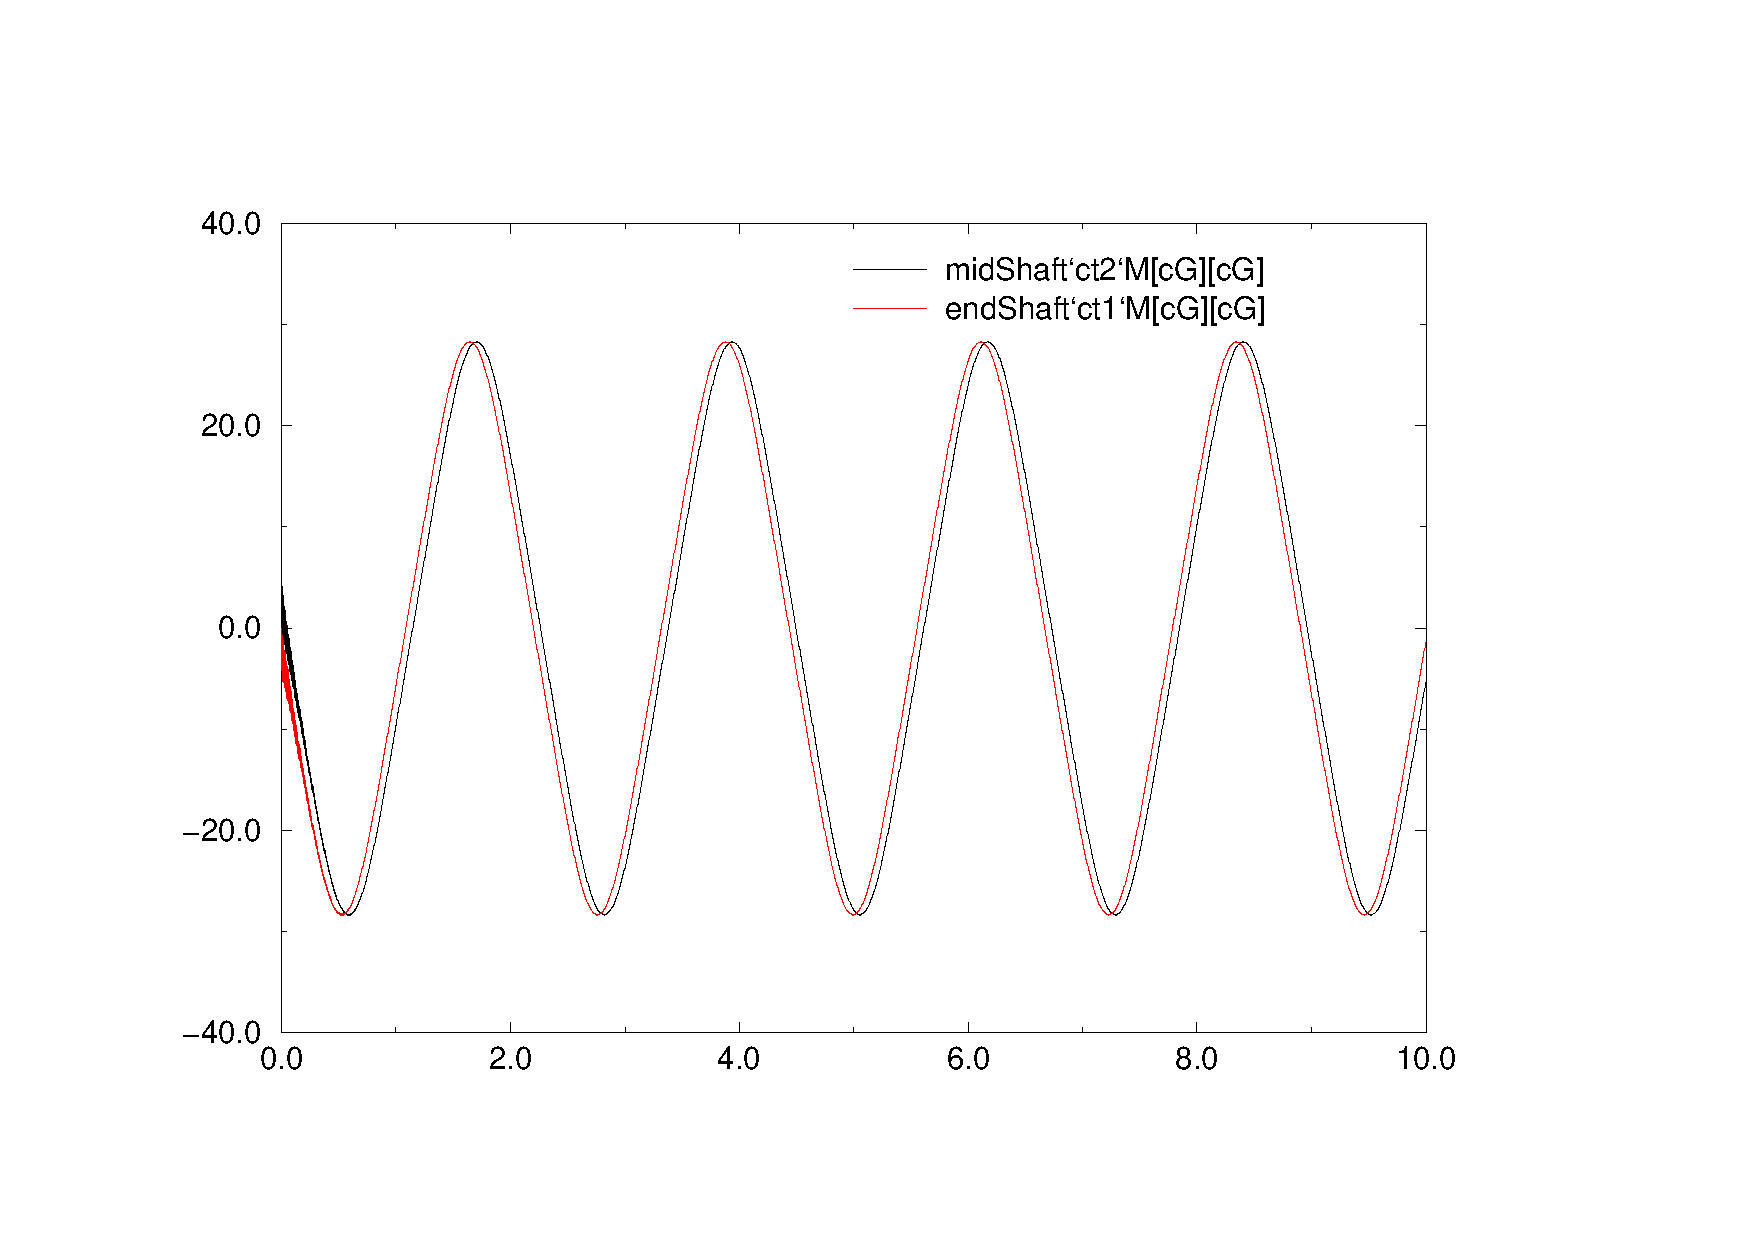
\includegraphics[width=6cm]{figs/S2S3_M.pdf}}
	\label{fig:MomentmidShaftendShaft}
     	}	
\caption{The difference in Moment between the TLM connected coordinate
	systems due to TLM delay.}
\label{fig:MomentShafts}
\end{figure}

Figure~\ref{fig:MomentShafts}, for instance, shows the moments created in the TLM interfaces of the connected Simulink models. 
One can nicely see the time delay in the connected interfaces due to TLM delay.

\section{Installation}
Generally the following steps need to be conducted for a correct installation of the plugin:
\begin{enumerate}
\item Install the plugin files on your system.
\item Add the installation directory or directories to the Matlab {\tt Search Path}.
\item Possibly adjust the StartTLMSimulink start-up script to your needs.
\end{enumerate}

The Simulink TLM-plugin consists of three files:
\begin{itemize}
\item A tlmforce S-Function, or tlmforce.mex* file.
\item A TLM library file, TLMLib.mdl.
\item A start-up script, StartTLMSimulink
\end{itemize}

The start script is located in the {\tt bin} directory in the TLMSimulator folder. 
The tlmforce S-Function mex and the TLMLib.mdl files are placed in the {\tt bin/\$ABI/Simulink} directory. 
There is a Linux and a MS-Windows version of the plugin available.

It is important that the TLMLib.mdl and tlmforce.mex* file are within the Matlab {\tt Search Path}. 
This can be achieved with the {\tt Select Path} dialog that can be opened from the {\tt File} menu in the Matlab main window.

Changes to the StartTLMSimulink script are typically not necessary. 
Note that there are two versions of the script, a MS Windows batch script and a c-shells script for Linux/Unix
systems. 
In case the system requires a special setup for running Matlab/Simulink it is recommended to make changes to the script. 
Below is the c-shell version of the script:
\begin{verbatim}
#!/bin/csh -f

setenv PATH ${PATH}:/home/alex/bin/matlab2006b/bin
set SIMCOMMAND="matlab -nosplash -nodesktop -nojvm -r"

#############################################################
#------ Changes below this line should not be needed     ----

if("a$1" == "a") then
echo This script is used by TLM manager to start simulations
echo It should result in a call to matlab/simulink
exit 1
endif

cd $1

echo Starting a simulation with input file: $6
echo Make sure that:
echo time = $2
echo timeEnd = $3
echo MaxTimeStep "<"= $4
echo Writing component name $1 and server name $5 to file tlm.config
echo $1 $5 > tlm.config
echo $2 $3 $4 >> tlm.config

echo Starting matlab/simulink
echo $SIMCOMMAND

echo Writing execution methods to runtlm.m
echo "$6;" > runtlm.m
if( "$4" != "0" ) then
 echo "opts = simset('MaxStep', $4);" >> runtlm.m
 echo "sim( '$6', [$2 $3], opts );" >> runtlm.m
else
 echo "sim( '$6', [$2 $3] );" >> runtlm.m
endif
echo "save; quit force;" >> runtlm.m

exec $SIMCOMMAND runtlm > ${6}.simlog
\end{verbatim}


\section{Creating External Simulink Models}
To enable an existing Simulink model for co-simulation is fairly simple:
\begin{enumerate}
\item Open the model and the TLM library TLMLib.mdl, see also Figure~\ref{fig:TLMLib}.
\item Drag the TLMForce (pure Simulink) or TLMInterface (SimMechanics) block into the model.
\item Create the necessary connections to the TLM block, see also Section~\ref{sec:TLMLib} for details about signal dimensions.
\item Send all signals of interest to the Matlab workspace or to a file.
\end{enumerate}

Remember, that the TLM plugin requires velocities to calculate output force and moment. 
Remember also, that all data must be expressed relative the global inertial system. 
Necessary coordinate transformations should be implemented in the Simulink model.

All external models are automatically executed on co-simulation start-up and terminated when the simulation is finished. 
Data that is not written to a file is lost when the simulation terminates. 
The Simulink plugin writes Matlab workspace content to the file {\tt matlab.mat} when the simulation is
finished. 
All simulation data that should be analyzed should either be written to a file during the simulation or stored in the workspace. 
The latter can be achieved by using a Simulink {\tt ToWorkspace} sink, by logging signals, or by logging Simulink {\tt Scope} data.

The next step is to create an external model from the TLM prepared Simulink model. 
It is created using the composite model editor. 
The composite model describes how different external models are connected and what TLM parameters should be used in the different TLM
connections. 
Creating external Simulink models is not different from creating any other external model. 
Only the correct start-up method, i.e., StartTLMSimulink needs to be selected.

{\em NOTE:} Neither Simulink nor SimMechanics can export surface graphics for visualization of the composite model. 
Graphics files, i.e., VRML or STL files, can be created from a CAD tool or with the Virtual-Reality authoring tool of the Matlab Virtual Reality toolbox.

Results from the co-simulation can be verified in CME by plotting the movement of the TLM interfaces.

\chapter{External BEAST Models}
\label{MMBEAST}
The TLM-Plugin has been implemented for BEAST. This section describes
how to integrate BEAST models into Meta-Models and Meta-Model
simulations.

\section{TLM Enabled BEAST models}
A BEAST model needs to be ``TLM enabled'' to participate in a
Meta-Model simulation. The TLM-plugin has been integrated into the
BEAST code and is thus always available in BEAST models.

Control-points are the interfaces for TLM connections in BEAST. One
can enable any fixed and flexible control-point in BEAST for TLM
connections. For TLM connections it is, however, recommended to use
control-points that are not connected to a tie.

Any BEAST model that has at least one TLM enabled control-point can
participate in a Meta-Model (co-)simulation. To enable a control-point
for TLM communication one needs to set the {\em TLMEnabledFlg} for
this control point in the following way:
\begin{itemize}
\item Right-click on the control point in the model-browser
\item From the pop-up menu select {\em Edit Variables...} and then
{\em TLM}
\item In the dialog set the {\em TLMEnabledFlg} to {\em Yes}.
\end{itemize}


The BEAST model can then be saved and integrated into as an external
model into a Meta-Model.


\section{BEAST Startup Script}
A startup script for running the BEAST simulation needs to be created
as well. A default script is distributed with the BEAST/MME
installation. It is called StartTLMBeast.bat.

{\bf Note:} The default \verb!StartTLMBeast.bat! Windows script needs to
be checked. This should probably be done together with a system
administrator and a member of the BEAST team. However below is a short
discussion of the script for advanced users.

Figure \ref{figStartBeast} presents a template for the start script.
The \verb!StartTLMBeast.bat! should first generate a file \verb!<CaseName>.tlm!
that will contain the parameter send to it by TLM manager.
Only the line giving start command for BEAST needs to be changed.

\begin{figure}[h]
\small{
\begin{verbatim}
@echo off
set BeastCmd="%BEAST%/bin/%ABI%/FORMAT-9.3/Beast_Serial"

echo execution directory is %1
cd %1

echo Starting a Beast simulation with input file: %6
echo Make sure that:
echo time = %2
echo timeEnd = %3
echo MaxTimeStep "<"= %4
echo Writing caseID %1 and server name %5 to file %6.tlm
echo %1 > %6.tlm
echo %5 >> %6.tlm
echo %2 >> %6.tlm
echo %3 >> %6.tlm
echo %4 >> %6.tlm

echo Starting beast
echo %BeastCmd% %6.in

%BeastCmd% %6.in > %6.simlog
\end{verbatim}
}
\caption{A template for the \emph{startadams.bat} script\label{figStartBeast}}
\end{figure}


\chapter{External Modelica Models}
\label{MMModelica}

In this chapter a description of how to design and co-simulate Modelica models with the TLM interface is given.

\subsection{Build and link TLM Manager to a Modelica tool}

The first step is to install the TLM manager. 
But please make sure you have Microsoft Visual Studio installed and the MinGW compiler for OMC and WSM (the MinGW compiler comes with OMC and WSM by default).

~\\Depending on which Modelica tool you are using, do as follows:

\subsubsection{In OpenModelica}
Run the script \textit{InstallTlmForOmc.bat} in MS DOS.

\subsubsection{In Wolfram SystemModeler}
Run the script \textit{InstallTlmForWsm.bat} in MS DOS.

\subsubsection{In Dymola}
Run the script \textit{InstallTlmForDymola.bat} in MS DOS.

~\\The above mentioned script files are located in \textit{\textbackslash TLMSimulator\textbackslash Modelica}.

~\\Note: The default Windows TLM installation BAT script may need some modifications.
The main issue is to modify the script file so the Modelica tool, Microsoft Visual Studio and the TLMSimulator folder paths are correct. 
Furthermore, it is important to add the TLMSimulator/bin folder path to the Windows System Environment Path. 
 

~\\ The installation script will set all the necessary paths in order to use the TLM interface. 
Thereafter, a library is generated and copied to the Modelica tool installation folder (for Dymola) or to the resource folder located in the TLMSimulator folder for OMC and WSM). 
For Dymola a tlmforce.h file is copied to the installation folder and for OMC and WSM the tlmforce.h file is copied to the resource folder. 
Next, the TLM Manager is compiled and built.

~\\In order to run the installation script simple start a commando prompt with administrator rights and execute the script.

~\\Before running the TLM Manager please check the log after executing the installation script for any errors. 
If the installation was a success restart the computer in order to update the System Environment paths.

\section{How to create a model with a TLM interface}
In this example we will split a model of a double pendulum and run a simulation with the TLM interface. 
The first step is to split the full model of the double pendulum and create two models, which are saved in two separate folders.

\image{!hbtp}{0.5}{path.png}{figuretext}{tableofcontentstext}

~\\In this example we will call the two new models 'DoublePendulum1' and 'DoublePendulum2'. 
At the end of each model (where the two models need to be connected) a TLM component is connected from the TLM Modelica library.

\subsubsection{Full model}
\image{!hbtp}{}{doublePendulum.png}{figuretext}{tableofcontentstext}

\subsubsection{Sub-model 1 (DoublePendulum1)}

\image{!hbtp}{}{doublePendulum1.png}{Sub-model 1 of a double Pendulum}{Sub-model 1 of a double Pendulum}

\subsubsection{Sub-model 2 (DoublePendulum2)}
\image{!hbtp}{}{doublePendulum2.png}{Sub-model 2 of a double Pendulum}{Sub-model 2 of a double Pendulum}

~\\When using the TLM interface in Modelica it is important to note that the TLM connection has to be connected to a body! Therefore, if you compare DoublePendulum2 with the full model, you can see that an extra body has been added. 
The extra body (boxBody1) is half of the boxbody1 from the full model (half mass and length). 
Furthermore, the boxBody1 from DoublePendulum1 is half (mass and length) of the boxbody1 from the full model.
It is important that the initial conditions for the objects are correct, i.e. the boxbody1 from DoublePendulum2 will have an initial position (r\textunderscore0[3] = {0.25,0,0})  for the given example.

\subsection{Prepare the XML composite model file for simulation }
In the XML file we have to define how the models are connected and which Modelica tool is used. 
Furthermore the simulation time is defined.
The XML file for the double pendulum: 
~\\
\image{!hbtp}{}{xml.png}{XML file for Modelica co-simulation}{XML file for Modelica co-simulation}

Save the file to the top folder (\textit{\textbackslash CompositeModels \textbackslash DoublePendulum}).

\subsection{Set up simulation settings}
The next step is to set up the simulation settings. 
For OpenModelica and Dymola all the simulation settings have to be modified in a BAT script. 
The BAT script is located in the bin folder: (\textit{\textbackslash TLMSimulator\textbackslash bin\textbackslash}).


\begin{itemize}
  \item For openModelica the file is called: \textit{StartTLMModelica.bat}.
  \item For Wolfram SystemModeler the file is called: \textit{StartTLMWSM.bat}.
  \item For Dymola the file is called: \textit{StartTLMDymola.bat}.
\end{itemize}

~\\The first step is to modify the Modelica tool installation path so it matches the user's installation folder on his computer. 
Following, the simulation function in the BAT script has to been updated. 
The function defines the simulations settings, i.e. tolerance, number of intervals, solvers etc. 
When using Wolfram SystemModeler the user doesn't need to modify the simulation settings. 
Using the Simulation Center, the user can follow the simulation 'live'.

\section{How to start a TLM simulation.}

To start a TLM simulation, follow these 5 steps (please note the paths below are relative and needs to be fully specified according to the TLMSimulator installation folder).

\begin{itemize}
  \item Start a commando prompt.
  \item Go to your CompositeModels folder, e.i. 
\textit{cd /TLMSimulator/CompositeModels/OmcOmcDoublePendulum/}
  \item To start the simulation run the following: \textit{tlmmanager.exe doublePendulum.xml}
\end{itemize}

~\\When the simulation is done the result files are located in the respective folders where the models are saved. 
The MAT files can now be loaded into the respective Modelica tools an analyzed.
\image{!hbtp}{}{doublePendulumResults.png}{Co-simulation of double pendulum results}{Co-simulation of double pendulum results}

~\\The blue plots are from the total model and the red are from DoublePendulum2. 
As can be seen, we have managed to carry out a parallel simulation with the TLM interface, and the results are almost identical. 
If the user wants to obtain better results, the 'Connection Form' parameters can be modified in the XML file to match the connection between the two TLM Modelica models even more accurately.



%\input{RunningMMCoSim}

\begin{thebibliography}{14}
%\addcontentsline{toc}{section}{References}

\bibitem{Johns-80}
	Johns, P.~B. and O'Brien, M.,
	{\em Use of the transmission-line modelling (t.l.m.) method to solve
  	non-linear lumped networks},
	The Radio and Electronic Engineer, 1980.

\bibitem{KrusDistrSim} Krus, P. and Jansson, A, {\em Distributed
	Simulation of Hydromechanical Systems}, Third Bath
	International Fluid Power Workshop, Bath, UK 1990

\bibitem{kim}
	Yongjoo, K. and Kyuseok, K. and Youngsoo S., and Taekyoon, A. and Kiyoung, C.,
  	{\em An integrated cosimulation environment for heterogeneous systems prototyping},
  	Design Automation for Embedded Systems, 1998

\bibitem{Stacke+Fritzson+Nordling-99}
	Stacke, L-E. and Fritzson, D. and Nordling, P., {\em BEAST---a
	rolling bearing simulation tool}, Proc. Instn Mech. Engrs,
	part K, Journal of Multi-body Dynamics, 1999

\bibitem{KrusModMech-99} Krus, P., {\em Modelling of Mechanical Systems
	Using Rigid Bodies and Transmission Line Joints}, Transactions
	of ASME, Journal of Dynamic Systems Measurement and
	Control. Dec 1999

\bibitem{Agrawal-2001} Agrawal A., Bakshi A., Davis J., Eames B., Ledeczi
	A., Mohanty S., Mathur V., Neema S., Nordstrom G., Prasanna
	V., Raghavendra, C., Singh M {\em MILAN: A Model Based
	Integrated Simulation Framework for Design of Embedded
	Systems}, Workshop on Languages, Compilers, and Tools for
	Embedded Systems (LCTES 2001), Snowbird, Utah, June 2001.

\bibitem{Ledeczi2001} A. Ledeczi, M. Maroti, A. Bakay, G. Karsai, J. Garrett,
	C. Thomason, G. Nordstrom, J. Sprinkle, P. Volgyesi, {\em The
	Generic Modeling Environment}, Proceedings of WISP'2001, May
	2001, Budapest, Hungary.

\bibitem{Fritzson} Fritzson, P. {\em Object-Oriented Modeling and
	Simulation with Modelica 2.1}, Wiley-Interscience, 2004

\bibitem{Siemers+Nakhimovski+Fritzson-05} Siemers, A. and Nakhimovski,
	I. and Fritzson, D., 
	{\em Meta-modelling of Mechanical Systems
	with Transmission Line Joints in Modelica}, Proceedings of the
	4th International Modelica Conference, Hamburg, Germany, 2005

\bibitem{Siemers+Fritzson-06} Siemers, A. and Fritzson, P. and  Fritzson, D., 
	{\em Meta-Modeling for Multi-Physics Co-Simulations applied
	for OpenModelica}, ANIPLA2006 International Congress on
	'Methodologies for Emerging Technologies in Automation',
	University of Rome "La Sapienza" ,November 13-14-15, 2006

\bibitem{Cogan-06}
	de Cogan, D. and O'Connor, W.J. and Pulko, S.,
	{\em Transmission Line Matrix in Computational Mechanics}.
	Taylor \& Francis, ISBN: 0-415-32717-2, 2006.

\bibitem{Siemers+Fritzson-07} Siemers, A. and Fritzson, D.,
	{\em A Meta-Modeling Environment for Mechanical System
	Co-Simulations}, The 48th Scandinavian Conference on
	Simulation and Modeling (SIMS 2007), Gothenburg
	(S\"{a}r\"{o}), Sweden, October 2007

\bibitem{Fritzson+Stahl+Nakhimovski-07} Fritzson, D. and St{\aa}hl,
	J. and Nakhimovski, I.  {\em Transmission line co-simulation
	of rolling bearing applications}, The 48th Scandinavian
	Conference on Simulation and Modeling (SIMS 2007), Gothenburg
	(S\"{a}r\"{o}), Sweden, October 2007

% \bibitem{Norling-07} Norling, K. and Broman, D. and Fritzson, P. and
% 	Siemers, A. and Fritzson D., {\em Secure Distributed
% 	Co-Simulation over Wide Area Networks}, The 48th Scandinavian
% 	Conference on Simulation and Modeling (SIMS 2007), Gothenburg
% 	(S\"{a}r\"{o}), Sweden, October 2007
I
% \bibitem{Pulko-90}
% 	Pulko, S.H. and Mallik, A. and Allen, R., and Johns, P.B.,
% 	{\em Automatic Timestepping in TLM Routines for the Modelling of Thermal
%   	Diffusion Processes}.
% 	Int. Journal of Numerical Modelling: Electronic Networks, Devices and Fields, 1990.

% \bibitem{Norling-08} Norling, K., {\em A performance Evaluation of
% 	Secure Distributed Co-Simulations over Wide Area Networks},
% 	Master Thesis, Link\"{o}ping University Electronic Press,
% 	Link\"{o}ping universitet, Sweden, 2008



% @article{ kim,
%   AUTHOR =       {Yongjoo Kim and Kyuseok Kim and Youngsoo Shin and Taekyoon Ahn and Kiyoung Choi},
%   TITLE =        "An integrated cosimulation environment for heterogeneous systems prototyping",
%   JOURNAL =      "Design Automation for Embedded Systems",
%   YEAR =         "1998",
%   volume =       "3",
%   number =       "2/3",
%   pages =        "163--186",
%   month =        Mar,
%   url = "citeseer.ist.psu.edu/kim98integrated.html",
%   url = "http://poppy.snu.ac.kr/papers/DAES98.pdf" }

%\bibitem{BML} Engelson, V., {\em BML Syntax and Semantic
%	Specification}, SKF Report, 2005

%\bibitem{IEEE1516} {\em High Level Architecture (HLA) - Framework and
%	Rules}, IEEE Standard for Modeling and Simulation, IEEE
%	1516-2000, Institute of Electrical and Electronics Engineers,
%	May 2000

%\bibitem{kuehl+weatherly+dahmann-99} Kuehl, F. and Weatherly, R. and
%	Dahmann, J., dahmann {\em Creating Computer Simulation
%	Systems, An Intruduction to the High Level Architecture},
%	Prentice Hall PTR, 1999

\bibitem{PtolemyII} {\em http://ptolemy.eecs.berkeley.edu/ptolemyII},
	Center for Hybrid and Embedded Software Systems (CHESS) in the
	Department of Electrical Engineering and Computer Sciences of
	the University of California at Berkeley.


%\bibitem{Dome} {\em http://www.htc.honeywell.com/dome}

%\bibitem{Lara+Vangheluwe} J. Lara, H. Vangheluwe, {\em Using AToM$^3$ as
%	a Meta-CASE Tool}, 4th International Conference on Enterprise
%	Information Systems, Ciudad Real, Spain

%\bibitem{Larsson+Johansson+Krus-2002} J. Larsson, B. Johansson,
%	P. Krus, M. Sethson, {\em MODLITH: A Framework Enabling
%	Tool-Independent Modelling and Simulation}, European
%	Simulation Symposium 2002, Dresden, Germany

%\bibitem{Engelson+Fritzson+Sellgren} V. Engelson, P. Fritzson,
%	U. Sellgren, {\em An Easy-to-use Generic Model Configurator
%	for Models in Multiple Tool Formats}, Proceedings of 5Th
%	EUROSIM Congress on Modelling and Simulation, September 2004,
%	Paris, France

%\bibitem{HOPSAN} {\em http://hydra.ikp.liu.se/hopsan.html}, Fluid and
%	Mechanical Engineering Systems (FluMeS) at the Department of
%	Mechanical Engineering (IKP) at Linköping University, Sweden

%\bibitem{Fritzson+Nordling-99} Fritzson, P. and Nordling, P.,
%	{\em Adaptive Scheduling Strategy Optimizer for Parallel
%	Rolling Bearing Simulation}, HPCN Europe `99, Amsterdam, April
%	1999

%\bibitem{Lee} Lee, E., {\em Model-Driven Development - From
%	Object-Oriented Design to Actor-Oriented Design}, Extended
%	abstract of an invited presentation at Workshop on Software
%	Engineering for Embedded Systems: From Requirements to
%	Implementation (a.k.a. The Monterey Workshop) Chicago,
%	Sept. 24, 2003

\bibitem{Cosimate} TNI-Software,
	{\em Cosimate co-simulation software},
	http://www.tni-software.com,
	Last visited on 14 February 2008

%\bibitem{MetaModelOrg} {\em http://www.metamodel.com}, Community site for meta-modeling and semantic modeling.

%\bibitem{MetaEdit} {\em http://www.metacase.com/mep}, MetaEdit+ website

\bibitem{MSC} MSC-Software,
	{\em MSC.ADAMS simulation software},
	http://www.mscsoftware.com, 
	Last visited on 14 February 2008
	
\bibitem{alachew2015} Mengist, A. and Asghar, A. and Pop, A. and Fritzson, P. and Braun, W. and Siemers, A. and Fritzson, D.
	 {\em An Open-Source Graphical Composite Modeling Editor and Simulation Tool Based on {FM}I and {TLM} Co-Simulation},
		Proceedings of the 11th International Modelica Conference, Versailles, France, September 2015

\end{thebibliography}


\end{document}
